%!TEX root = ../Thesis.tex
\section{Dokumentation der Software}
\fancyhead[R]{Dokumentation der Software}
\label{instal}

\subsection{Dokumentation der Paketstruktur (Sertan Cetin)}
%%%%%%%%%%%
%Sertan
%%%%%%%%%%%
Die entwickelte App ist innerhalb des Paketes com.example.robin.angrynerds-wip in mehrere Klassen unterteilt. Zu jeder Activity gehören mehrere Klassen. Um die Übersichtlichkeit zu steigern, wurden die Klassen und Activities in Ordnern untergebracht. Die gesamte Ordnerstruktur sieht wie folgt aus:

\begin{figure}[H]
\centering
\begin{minipage}[t]{1\textwidth} % Breite, z.B. 1\textwidth		
\caption{Paketstruktur} % Überschrift
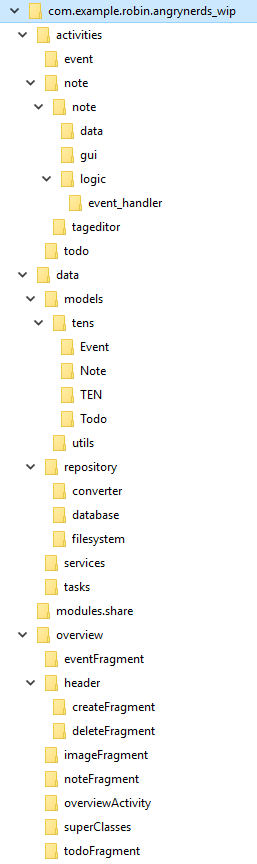
\includegraphics[width=5.5cm]{img/Projektordnerstruktur}\\ % Pfad
\source{Erstellt von Sertan Cetin} % Quelle
\end{minipage}
\end{figure}

Das Paket beinhaltet insgesamt fünf Activities mit jeweils einer ApplicationLogic, Gui und Data.

\begin{figure}[H]
\centering
\begin{minipage}[t]{1\textwidth} % Breite, z.B. 1\textwidth		
\caption{Paketstruktur} % Überschrift
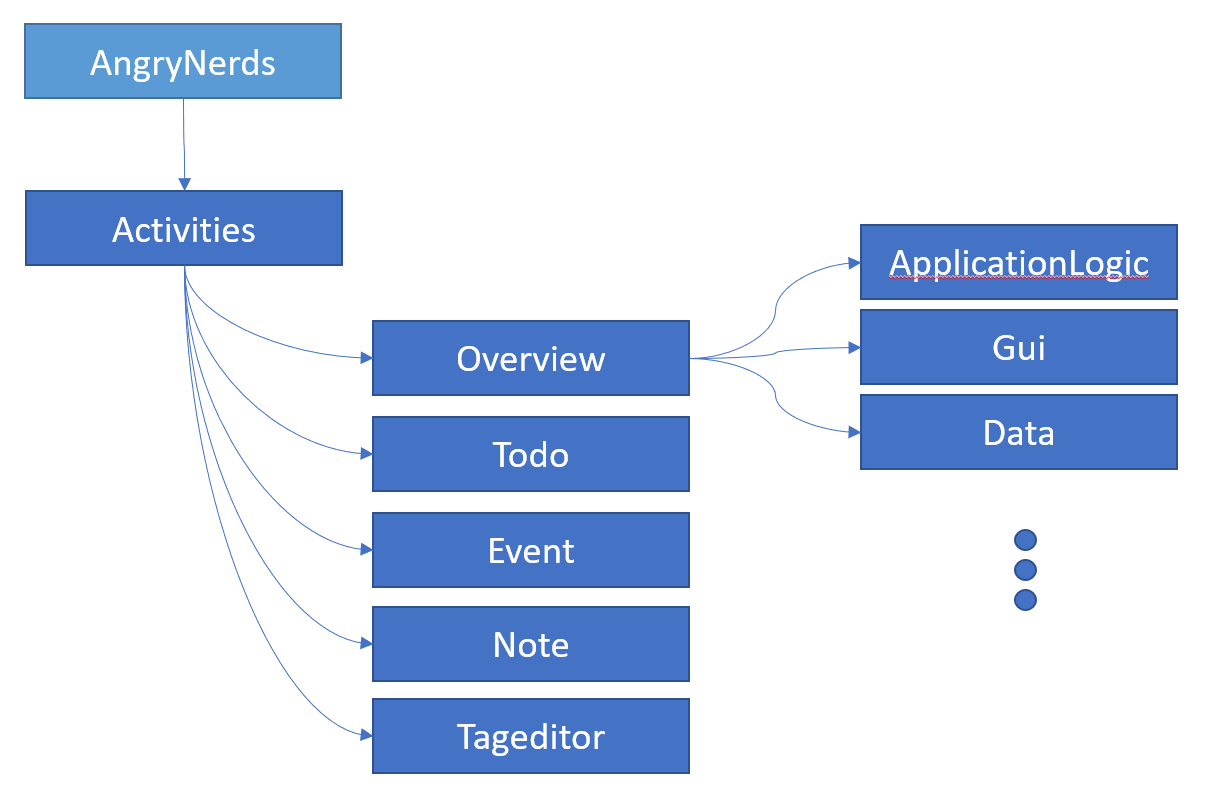
\includegraphics[width=1\textwidth]{img/Paketstruktur}\\ % Pfad
\source{Erstellt von Sertan Cetin} % Quelle
\end{minipage}
\end{figure}

\newpage
\subsection{Dokumentation der Activities}
%%%%%%%%%%%
%Alle
%%%%%%%%%%%

\subsubsection{Main Activity}
\fancyhead[L]{Main Activity}

%Yannick
\paragraph{Aufgabe und Funktionen (Yannick Rüttgers)}
Die in diesem Kapitel erläuterte Activity Overview dient dem Nutzer als Einstiegspunkt in die Applikation. Von hier aus werden alle weiteren Activities aufgerufen.

Wenn der Nutzer die Applikation startet, sieht er als erstes diese Activity. Diese enthält alle bereits erstellten TENs in Kachelform mit einigen Infos. Die Kacheln sind in einer oder mehreren Spalten, je nach Größe des Displays angeordnet. Diese Kacheln sind scrollbar.

Am unteren Bildschirmrand hat der Nutzer die Möglichkeit, sich nur die Kacheln, die zu einer der verschiedenen TEN-Arten gehören, anzeigen zu lassen. Dazu gibt es vier Buttons, die die jeweiligen TEN-Arten und eine generelle Übersicht über alle TENs darstellen.

Am oberen Bildschirmrand kann der Nutzer die einzelnen TEN-Arten neu erstellen, oder eine Suche öffnen. Auch hier sind wieder Buttons zu finden.

Der Nutzer hat die Möglichkeit, über ein langes gedrückt halten einer Kachel, in den Löschmodus zu gelangen. Hier können dann multiple Kacheln markiert werden und über ein neues Menü am oberen Bildschirmrand gelöscht werden.

Weitere Infos und Screenshots zum Layout der Applikation sind im nachfolgenden Kapitel zu finden.

Da die Activity als Einstiegspunkt in die Applikation genutzt wird, müssen von hier aus alle weiteren Activities zu erreichen sein. Die weiteren Activities umfassen die Anzeige und Neuerstellung von TENs. Die Erreichung dieser geschieht über die vorhin genannten Buttons und über die Kacheln.

Die Activity selbst besteht aus einer Oberfläche mit den genannten Buttons. Die einzelnen TENs werden mithilfe von Fragments eingefügt. Für jede TEN-Art gibt es ein eigenes Fragment. Diese Fragments bestehen aus mehreren Klassen. Der genaue Aufbau dieser wird später erläutert. Um mit den Fragments arbeiten zu können, verfügt die Activity über verschiedene Helferklassen, um diesen Prozess zu strukturieren.


%Fabia
\paragraph{Layouts, Screenshots (Fabia Schmid)}
Das Layout der Overview Activity orientiert sich an dem vorher erstellten Mockup und besteht aus drei Grundkomponenten. Es gibt am oberen Bildschirmrand eine Leiste zum Erstellen von Notes, Events und ToDos, sowie ein Button zum Suchen. Unter dieser leiste befindet sich ein Container, welcher die verschiedenen Fragments der vorhandenen Notes, Events und ToDos beinhaltet. Am unteren Bildschirmrand befindet sich noch eine Leiste mit vier Buttons zum Filtern der  Fragments (vgl. Abbildung Overview Activity).

Die obere Leiste ist ein RelativeLayout, welches eine TextView und drei Button beinhaltet. Diese ist ein gesondertes Fragment, damit der Wechsel zu einer anderen Leiste, z.B. bei dem Löschvorgang, vereinfacht wird. Darunter ist eine ScrollView, die es ermöglicht, dass durch die Fragments gescrollt werden kann. In der ScrollView befinden sich LinearLayouts, die mit den Fragments befüllt werden können. Die untere Leiste besteht abschließend aus einem LinearLayout, welches horizontal ausgerichtet ist und vier Buttons beinhaltet, mit denen gefiltert werden kann.

\begin{figure}[H]
\centering
\begin{minipage}[t]{1\textwidth} % Breite, z.B. 1\textwidth		
\caption{Overview Activity} % Überschrift
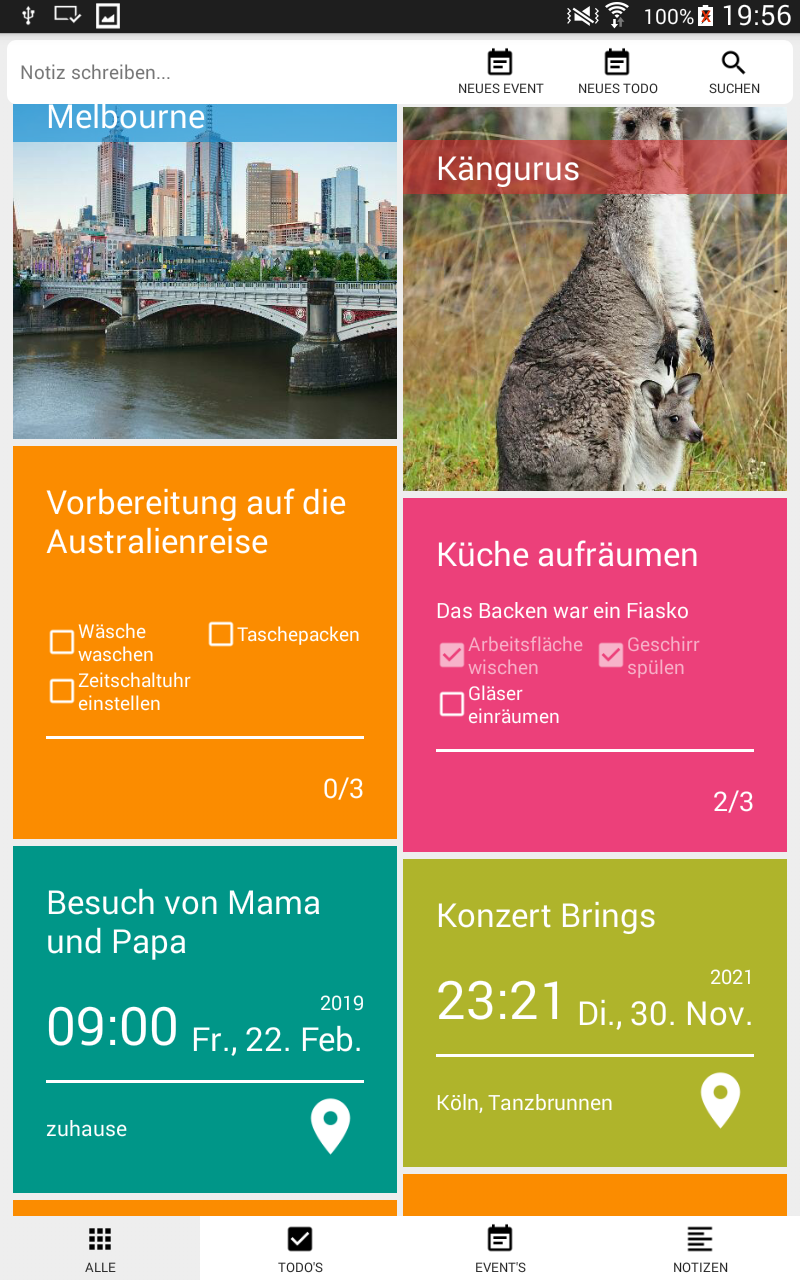
\includegraphics[height=20cm]{img/Overview}\\ % Pfad
\source{Screenshot aus der Benutzeroberfläche} % Quelle
\end{minipage}
\end{figure}

Die Activity Overview zeigt normal 2 Spalten mit Fragments, wenn jedoch das Tablet gedreht wird zeigt die Landscape-Ansicht drei Spalten mit Fragments, um den Bildschirm optimal zu nutzen (vgl. Abbildung Landscape-Ansicht Overview Activity).

\begin{figure}[H]
\centering
\begin{minipage}[t]{1\textwidth} % Breite, z.B. 1\textwidth		
\caption{Landscape Ansicht - Overview Activity} % Überschrift
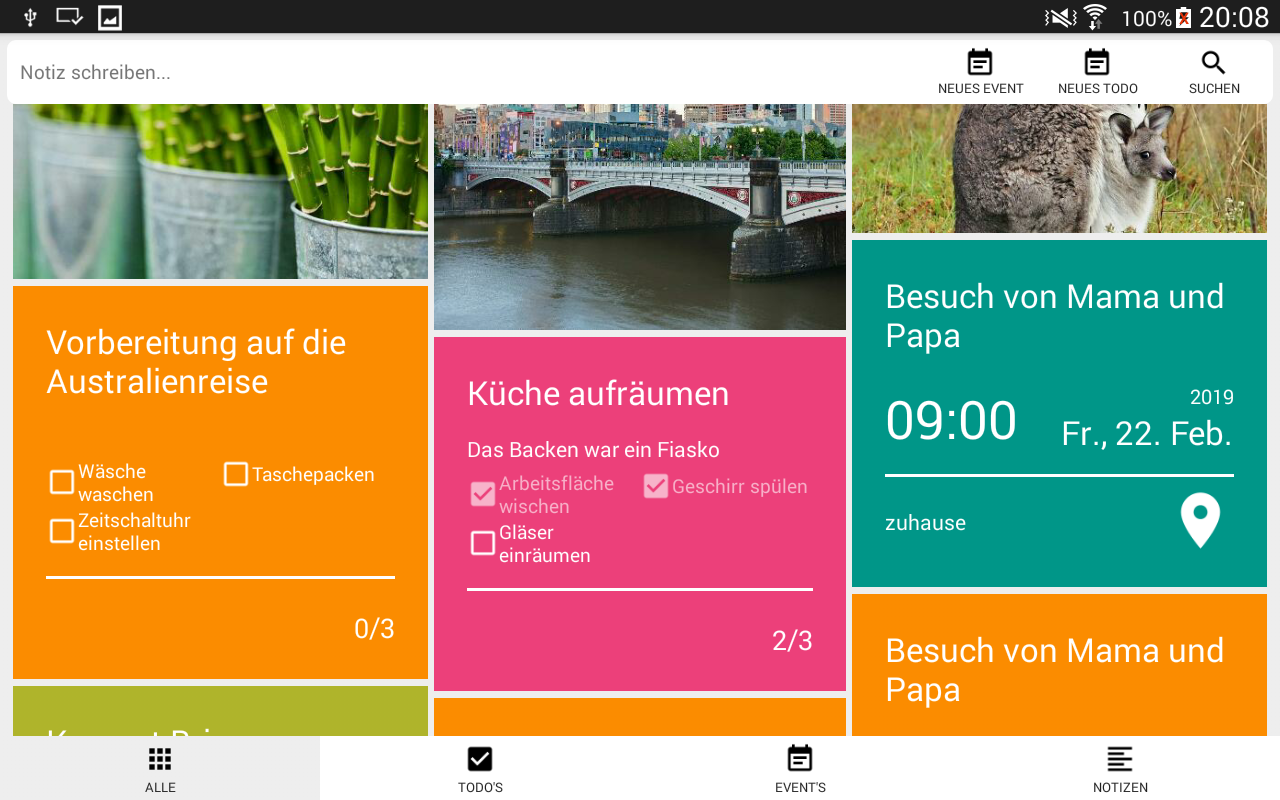
\includegraphics[width=1\textwidth]{img/Landscape}\\ % Pfad
\source{Screenshot aus der Benutzeroberfläche} % Quelle
\end{minipage}
\end{figure}

Die drei verschiedenen Arten von Fragments sind Notes, ToDo und Event.

Bei einer Note wird die Überschrift und ein Textauszug angezeigt. Wenn jedoch ein Bild in der Notiz vorhanden ist wird dieses mit der Überschrift in der Overview Activity angezeigt (vgl. Abbildung Note Fragments).

\begin{figure}[H]
\centering
\begin{minipage}[t]{1\textwidth} % Breite, z.B. 1\textwidth		
\caption{Note Fragments} % Überschrift
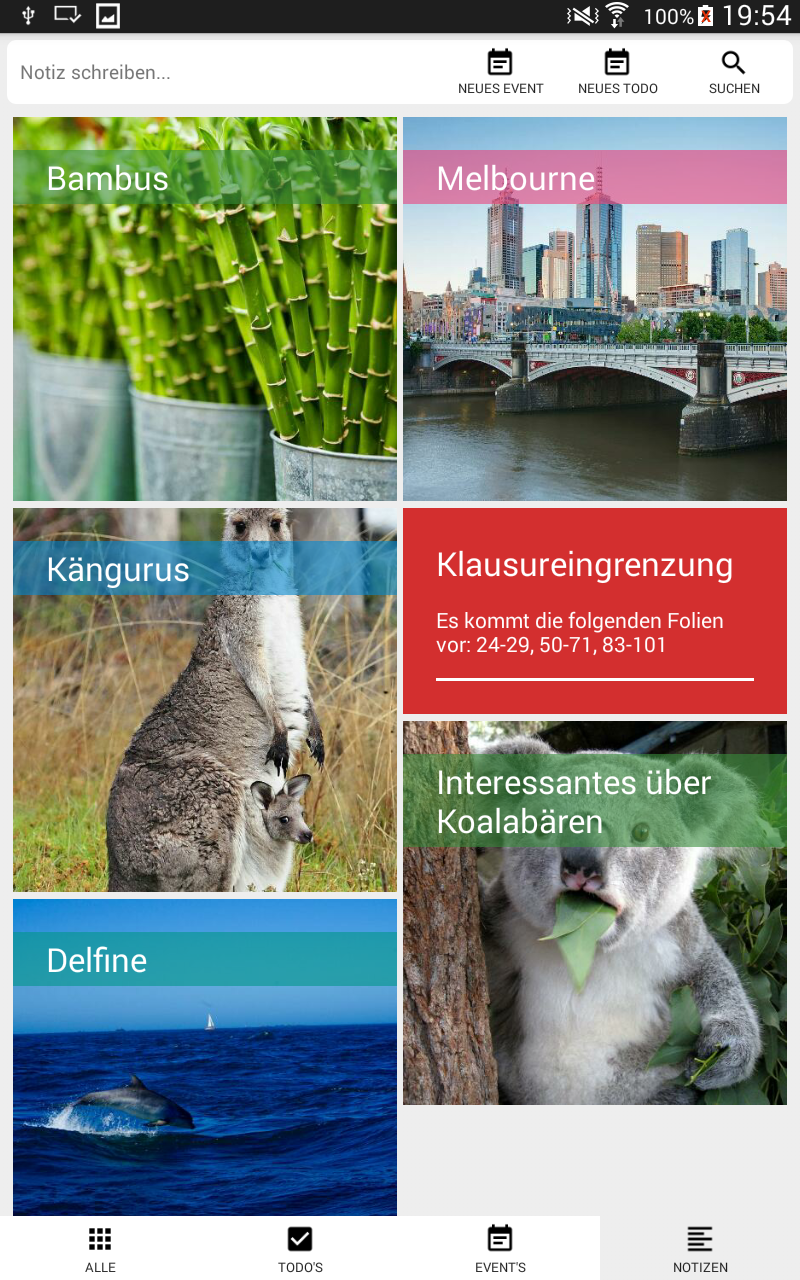
\includegraphics[height=17cm]{img/FragmentN}\\ % Pfad
\source{Screenshot aus der Benutzeroberfläche} % Quelle
\end{minipage}
\end{figure}

Die Fragments für die ToDos, zeigen auch den Titel an und die einzelnen Aufgaben mit Kästchen, die mit einem Hacken gefüllt sind, wenn sie erledigt sind. Zusätzlich wird Angezeigt, wie viele Aufgaben schon erfüllt wurden (vgl. Abbildung ToDo Fragments).

\begin{figure}[H]
\centering
\begin{minipage}[t]{1\textwidth} % Breite, z.B. 1\textwidth		
\caption{Todo Fragments} % Überschrift
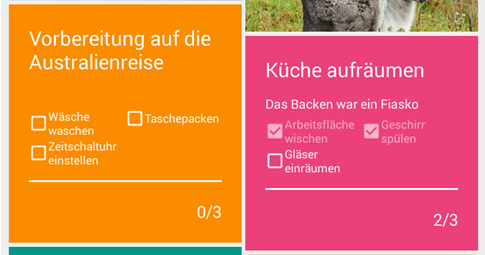
\includegraphics[width=1\textwidth]{img/FragmentT}\\ % Pfad
\source{Screenshot aus der Benutzeroberfläche} % Quelle
\end{minipage}
\end{figure}

Die Event Fragmentes bestehen aus der Überschrift, dem Datum und der Uhrzeit, sowie aus einem Ort, der angegeben werden kann (vgl. Abbildung Event Fragments).

\begin{figure}[H]
\centering
\begin{minipage}[t]{1\textwidth} % Breite, z.B. 1\textwidth		
\caption{Event Fragments} % Überschrift
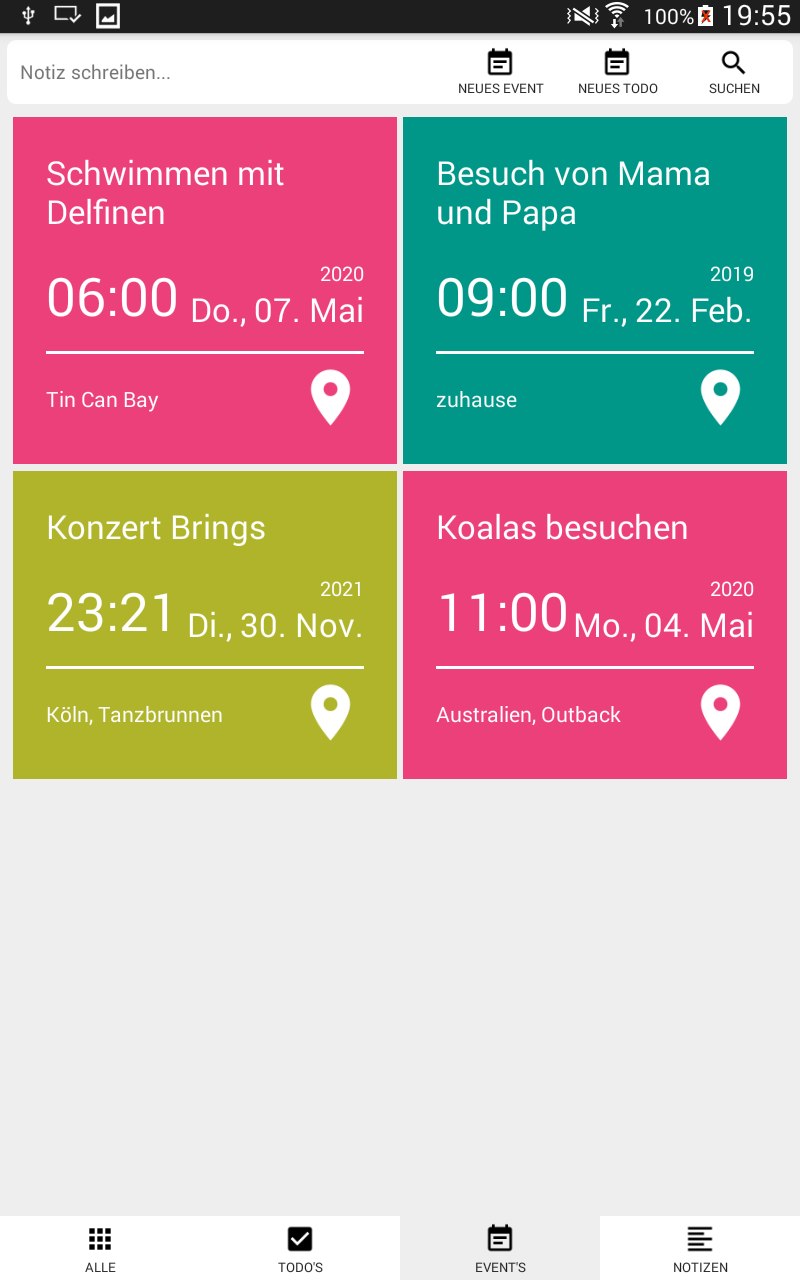
\includegraphics[height=17cm]{img/FragmentE}\\ % Pfad
\source{Screenshot aus der Benutzeroberfläche} % Quelle
\end{minipage}
\end{figure}

In der Overview Activity kann zusätzlich gesucht und gelöscht werden. Wenn man einen langen Click auf ein Fragment macht, wird die obere Leiste verändert und man bekommt einen Button zum Löschen. Dies ist dadurch möglich, dass die obere Leiste ein Fragment ist. Zusätzlich kann in dieser Ansicht nun auf die verschiedenen Fragments geklickt werden, um diese zu markieren und mehrere gleichzeitig zu löschen. Markierungen werden mittels einem Hacken gekennzeichnet. Diese Ansicht kann durch den Zurück-Pfeil verlassen werden (vgl. Abbildung Overview Activity Löschen).

\begin{figure}[H]
\centering
\begin{minipage}[t]{1\textwidth} % Breite, z.B. 1\textwidth		
\caption{Overview Activity - Löschen} % Überschrift
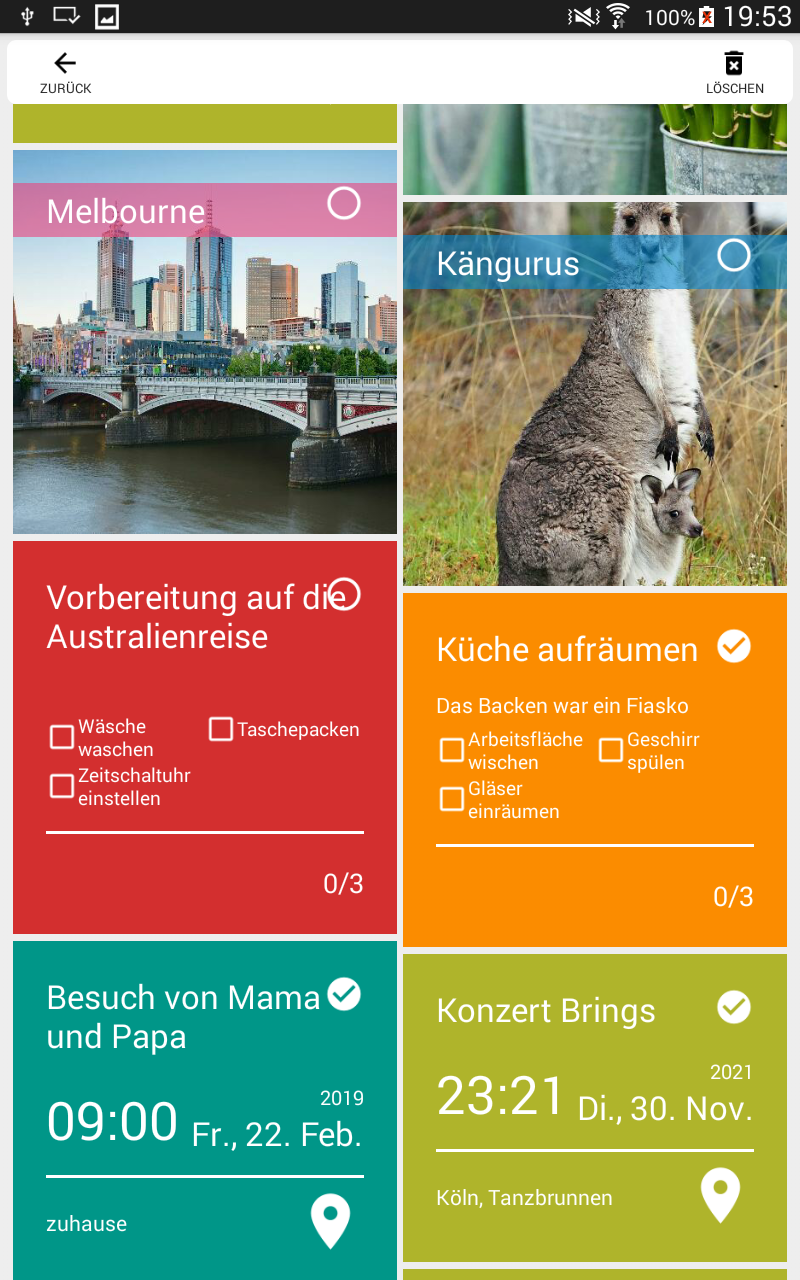
\includegraphics[height=17cm]{img/Loeschen}\\ % Pfad
\source{Screenshot aus der Benutzeroberfläche} % Quelle
\end{minipage}
\end{figure}

Auch bei der Suchfunktion wird die obere Leiste angepasst. Auch hier möglich ducrh das Fragment. Dabei kann nun ein beliebiges Wort eingegeben werden, welches in den verschiedenen Einträgen gesucht wird. Die gefundenen Einträge werden daraufhin angezeigt. Um die Suche zu beenden kann der Zurück-Pfeil verwendet werden (vgl. Abbildung Overview Activity Suchen).

\begin{figure}[H]
\centering
\begin{minipage}[t]{1\textwidth} % Breite, z.B. 1\textwidth		
\caption{Overview Activity - Suchen} % Überschrift
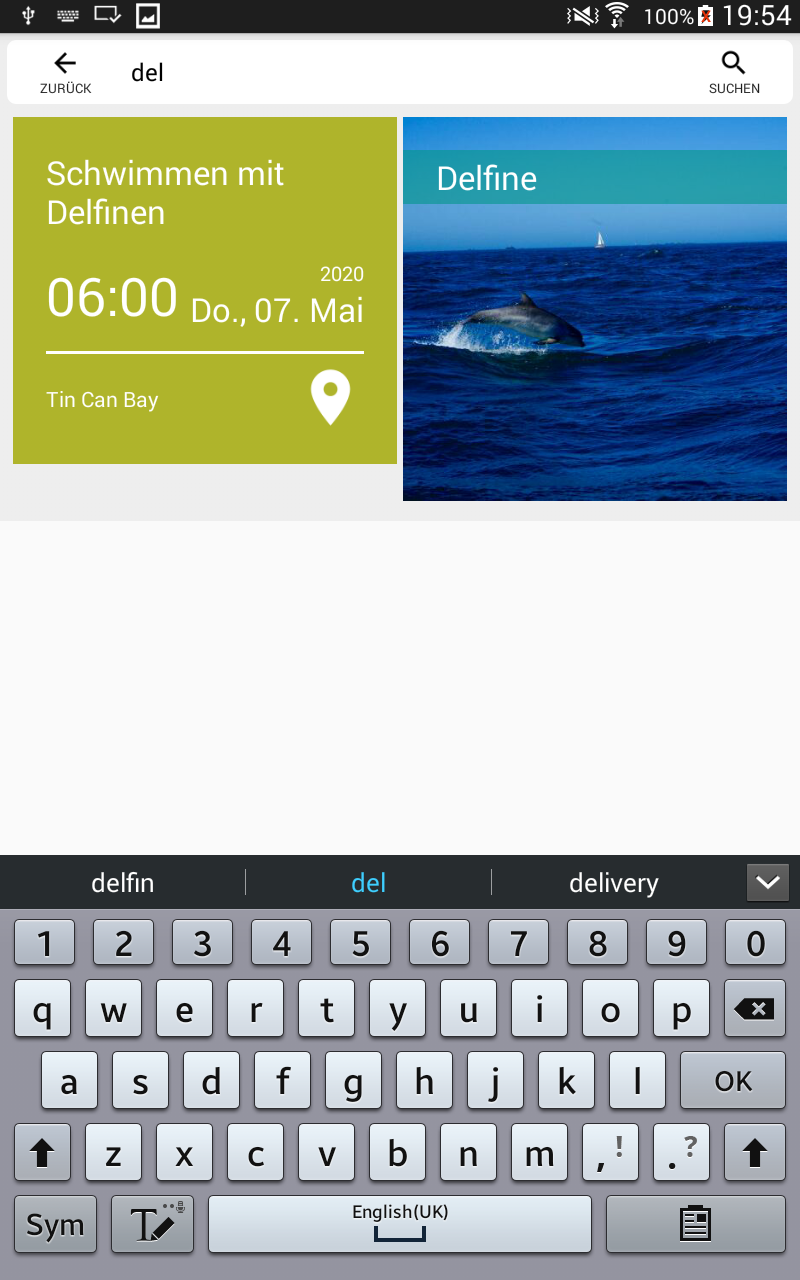
\includegraphics[height=17cm]{img/Suchen}\\ % Pfad
\source{Screenshot aus der Benutzeroberfläche} % Quelle
\end{minipage}
\end{figure}

%Yannick
\paragraph{Use Case (Yannick Rüttgers)}
Wie bereits geschrieben, dient diese Activity dem Nutzer als Einstiegspunkt in die Applikation. Hier kann er einige Aktionen durchführen.
 
Zum einen kann er die Oberfläche der Übersicht selbst beeinflussen. Hierzu gibt es am unteren Bildschirmrand einige Buttons, mit denen er nach den verschiedene TEN-Arten filtern kann. Zusätzlich kann er über eine Suchfunktion alle TENs durchsuchen.

Aus dieser Activity heraus können vom User auch neue TENs erstellt werden. Hierzu wird er allerdings an weitere Activities weitergeleitet.

Zuletzt ist es dem Nutzer auch möglich, mehrere TENs auf einmal zu löschen. Dies geschieht, wie bereits gesagt, über ein markieren einzelner Kacheln.

Im Folgenden ist das Usecase-Diagramm für die Übersicht zu sehen.

\begin{figure}[H]
\centering
\begin{minipage}[t]{1\textwidth} % Breite, z.B. 1\textwidth		
\caption{Usecase Diagramm der Overview} % Überschrift
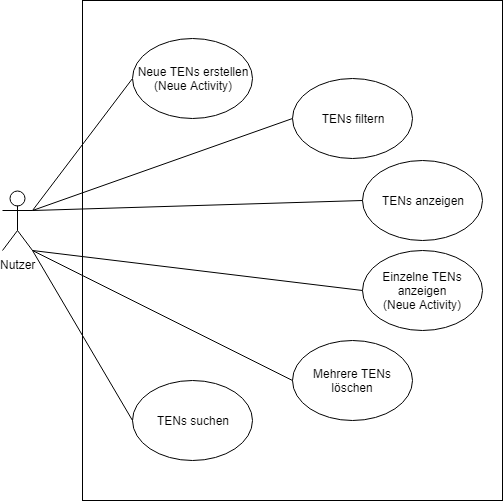
\includegraphics[width=1\textwidth]{img/Usecase_Overview}\\ % Pfad
\source{Erstellt von Yannick Rüttgers} % Quelle
\end{minipage}
\end{figure}

%Yannick
\paragraph{Datenstruktur und Typen (Yannick Rüttgers)}
Die Daten für diese Activity werden hauptsächlich über die Klasse OverviewData verwaltet.

Wenn die Activity initiiert wird, werden zuerst alle nötigen Instanzen erstellt. Hierzu gehört unter anderen eine Instanz der Klasse OverviewData. Diese Klasse ruft in ihrem Konstruktor mithilfe einer statischen Servicemethode alle TENs als Objekte ab. Diese Objekte werden in einer ArrayList gespeichert. Bei Bedarf werden diese Daten neu geladen.

Um beim Suchen oder Filtern nicht alle Daten neu laden zu müssen, gibt es eine weitere ArrayList, die immer den gefilterten Datenstand enthält. Aus diesen Daten werden die Fragments generiert.

Um die Filterung von Fragments beim Wechsel der Orientierung der Applikation beibehalten zu können, wird dies ebenfalls im Dataobjekt hinterlegt.

Wenn Fragments generiert werden, bekommen diese die Daten des zugehörigen TEN-Objekts als Bundle mitgegeben. Während der Initialisierung jedes Fragments, werden die Daten im jeweiligen Data Objekt abgelegt. Die Parameter dieser Dataobjekte bilden zum größten Teil die der TEN-Objekte ab. Im Konstruktor der Dataklasse werden den einzelnen Parametern dann die Werte aus dem Bundle zugewiesen. Da in der Activity die TENs nicht bearbeitet werden können, gibt es im Nachhinein keine Möglichkeit den Fragments neue Daten zuzuweisen.

Zusätzlich hält jedes Fragment zwei Informationen über sich. Dies ist zum einen der Löschzustand, über den das Fragment steuern kann, ob es zum Löschen markiert werden kann oder nicht. Zum anderen hält das Fragment die Information, ob es markiert ist, um dies im Falle einer Löschung angeben zu können. Diese beiden Informationen können aus dem Fragment abgerufen werden.

%Yannick
\paragraph{Dokumentation des Quelltextes der Activity (Yannick Rüttgers)}

\subparagraph{Allgemein}

Die OverviewActivity besteht aus 35 verschiedenen Klassen. Diese Klassen sind in verschiedene Pakete unterteilt.

Zum einen gibt es die Klassen, die unmittelbar zur OverviewActivity an sich gehören. Zu diesen zugehörig sind die Klassen, die für den Header der Activity genutzt werden.

Alle weiteren Klassen werden für die Fragments, die die TENs darstellen, genutzt. Hierzu gibt es vier Superklassen und zwei Listener, die in allen Fragments genutzt werden. Jedes der vier verschiedenen Fragments hat nochmal vier weitere Klassen, die von den Superklassen erben.
In Folgender Grafik soll dies verdeutlicht werden.

\begin{figure}[H]
\centering
\begin{minipage}[t]{1\textwidth} % Breite, z.B. 1\textwidth		
\caption{Klassendiagramm} % Überschrift
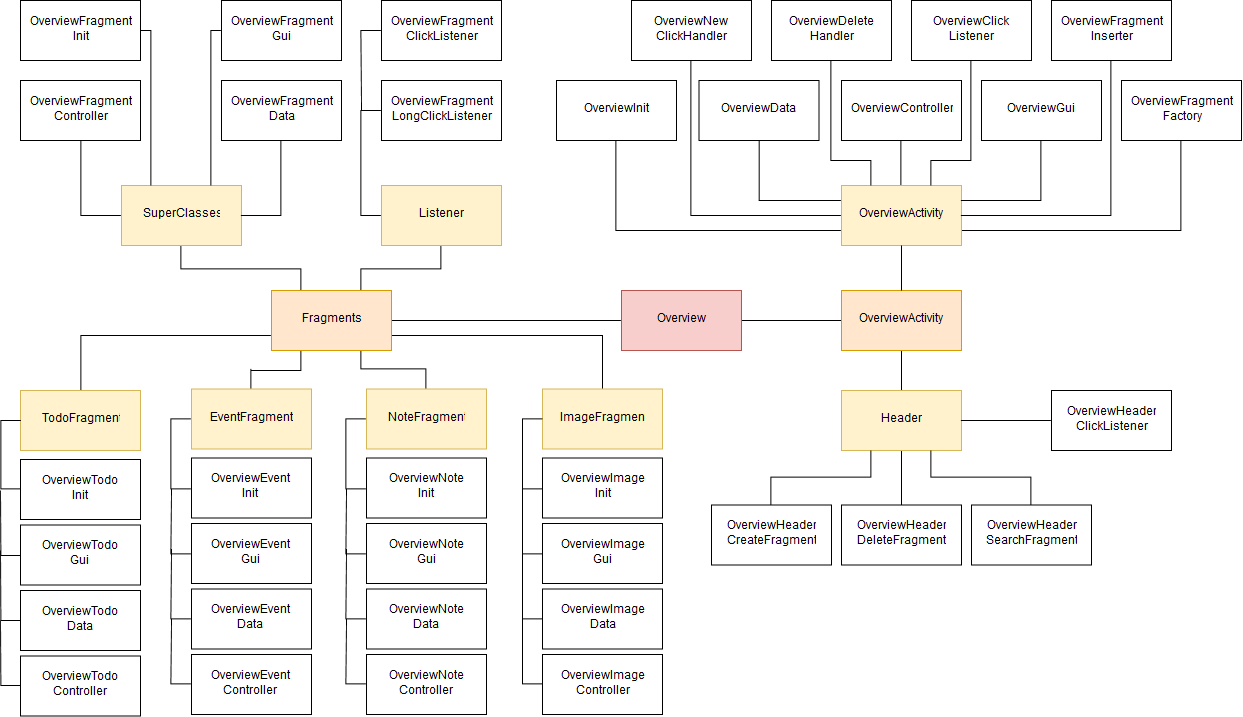
\includegraphics[height=20cm]{img/Klassendiagramm_lite}\\ % Pfad
\source{Erstellt von Yannick Rüttgers} % Quelle
\end{minipage}
\end{figure}

Die Funktion der Klassen und wichtige Methoden werden im Folgenden erläutert.

\subparagraph{Activityklassen}

Zu den Klassen, die unmittelbar zur Activity gehören, zählen neun verschiedene Klassen.

\subparagraph*{Klasse: class OverviewInit extends AppCompatActivity}

Diese Klasse ist für die Initialisierung der verschiedenen Komponenten der Activity zuständig. Da sie von der Superklasse AppCompatActivity erbt, implementiert sie zusätzlich die Methoden des Activitylifecycles.

Wichtige Methoden:

\textit{-protected void OnCreate(Bundle savedInstanceState)}

Diese Methode ist eine der Lifecyclemethoden von Activities, sie wird beim entstehen der Activity aufgerufen. Hier werden die verschiedenen Komponenten der Activity mit den zugehörigen Methoden initiiert.

\textit{-public void onConfigurationChanged(Configuration newConfig)}

Diese Methode wird aufgerufen, wenn sich etwas an der Konfiguration der Applikation ändert, wie in diesem Fall die Ausrichtung des Gerätes. Hier werden der Controller und die Gui neu initiiert. Dazu werden die Methoden initGui() und initController() aufgerufen.

\subparagraph*{Klasse: class OverviewData}

Diese Klasse ist für die Datenhaltung innerhalb der Activity verantwortlich. Hier befinden sich auch die zum Sortieren und zum Suchen verwendeten Methoden. Initial werden die Daten einmal geladen, bei Bedarf werden diese über eine Methode neugeladen. Die Daten werden dabei zweimal gehalten: Eine Liste enthält alle TENs, die andere Liste enthält die TENs, die angezeigt werden sollen.

Wichtige Methoden:

\textit{-public void refresh()}

Läd die Daten neu.

\textit{-public ArrayList<TEN> filterData()}

Filtert die Daten nach dem aktuell ausgewählten TEN-Typen.

\textit{-public void search(String pSearchString)}

Fügt nur die Suchergebnisse in die Liste der TENs ein, die angezeigt werden sollen.

\subparagraph*{Klasse: class OverviewGui}

Diese Klasse verwaltet die Benutzeroberfläche der Activity.

Wichtige Methoden:

\textit{-public void markButton(Class pClass)}

Markiert einen der Buttons am unteren Bildschirmrand, je nachdem welcher TEN-Typ ausgewählt ist.

\textit{-public void showFooter() / hideFooter()}

Zeigt oder versteckt die Buttons am unteren Bildschirmrand.

\subparagraph*{Klasse: class OverviewController}

Diese Klasse verwaltet die einzelnen Helferklassen und stellt die Logik der Activity da. 

Wichtige Methoden:

In der Klasse wird die Suche aktiviert, sowie das Löschen von TENs verwaltet. Hierzu werden die Helferklassen OverviewDeleteHandler, OverviewNewClickHandler, OverviewFragmentFactory und OverviewFragmentInserter genutzt. 

\subparagraph*{Klasse: class OverviewFragmentFactory}

Diese Klasse erstellt verschiedene Arten von Fragments, die dann später genutzt werden können.

Wichtige Methoden:

\textit{-public Fragment createHeader(Create/Delete/Search)Fragment()}

Diese Methode liefert das gewählte Headerfragment zurück.

\textit{-public ArrayList<Fragment> createTENFragments(ArrayList<TEN> pTENs)}

Erstellt eine Liste von Fragments, die aus den TENs erstellt werden. Je nach Art des TENs wird ein unterschiedliches Fragment erstellt.

\subparagraph*{Klasse: class OverviewFragmentInserter}

Diese Klasse fügt Fragments in die Benutzeroberfläche ein. Hierzu wird der FragmentManager der Activity genutzt.

Wichtige Methoden:

\textit{-public void insertFragment(int pContainerID, Fragment pFragment, String pTag)}

Fügt ein Fragment in einen gewählten Container ein. Dem Fragment wird ein Tag zugewiesen.

\textit{-public void replaceFragment(int pContainerID, Fragment pFragment, String pTag)}

Ersetzt ein Fragment in einem gewählten Container durch ein anderes. Dem Fragment wird ein Tag zugewiesen.

\textit{-public void insertFragments(int[] pContainerIDs, ArrayList<Fragment pFragments)}

Fügt eine beliebige Anzahl Fragments in eine beliebige Anzahl Container an. Dabei werden die Container zyklisch durchlaufen.

\subparagraph*{Klasse: class OverviewClickListener}

Diese Klasse verwaltet die Klickevents der OverviewActivity. Je nach geklicktem Button wird eine andere Methode des Controllers aufgerufen.

Wichtige Methoden:

\textit{-public void onClick(View view)}

Ruft je nach angeklickter View die show()-Methode des Controllers mit einem bestimmten Parameter auf.

\subparagraph*{Klasse: class OverviewDeleteHandler}

Diese Klasse verwaltet die Methoden, die zum Löschen beziehungsweise nicht Löschen von TENs nötig sind.

Wichtige Methoden:

\textit{-public void longClick()}

Aktiviert den Löschvorgang für alle Fragments.

\textit{-public void back()}

Deaktiviert den Löschvorgang für alle Fragments.

\textit{-public void delete()}

Sammelt alle markierten Fragments und löscht die dazugehörigen TENs. Deaktiviert den Löschvorgang für alle anderen Fragments.

\subparagraph*{Klasse: class OverviewNewClickHandler}

Verwaltet das Erstellen von neuen TENs.

Wichtige Methoden:

\textit{-public void newTEN(Class pClass)}

Startet eine neue Activity, je nachdem welche TEN-Art angegeben wurde.

\subparagraph{Header}

Die Header der Activity sind wechselnde Fragments, die verschiedene Aufgaben haben. Sie werden am oberen Bildschirmrand ausgetauscht. Ein Fragment dient dem Neuerstellen von TENs, eines das Löschen und eines das Suchen.

Die Fragments teilen sich einen ClickListener.

\subparagraph*{Klasse: class OverviewHeaderCreateFragment}

Dieses Fragment dient dazu, das Erstellen von neuen TENs anzustoßen. Hierzu enthält es drei Buttons. Zusätzlich gibt es einen Button zum Starten der Suche.

\subparagraph*{Klasse: class OverviewHeaderDeleteFragment}

Dieses Fragment dient dem Löschvorgang. Es gibt einen Button zum Abbrechen des Prozesses und einen Button, um die Löschung durchzuführen.

\subparagraph*{Klasse: class OverviewHeaderSearchFragment}

Dieses Fragment dient dem Suchvorgang. Es gibt ein Textfeld, in das ein Suchbegriff eingegeben werden kann. Außerdem gibt es einen Button zum Abbrechen des Prozesses und einen, um die Suche durchzuführen.

\subparagraph*{Klasse: class OverviewHeaderClickListener}

Diese Klasse behandelt die Clickevents der Headerfragments. Je nachdem, welcher Button in einem der Fragments geklickt wurde, wird eine andere Methode im Controller aufgerufen.

Wichtige Methoden:

\textit{-public void onClick(View view)}

Diese Methode wird ausgeführt, sobald einer der Buttons eines Headers geklickt wird. Je nachdem, welcher Button dies war, wird eine Methode im Controller aufgerufen.

\subparagraph{Superklassen}

Die folgenden Klassen dienen als Superklassen für die Fragments. Dies wurde so entwickelt, da alle vier Fragments sich ähnliche Funktionen teilen. Große Teile der Implementierung nutzen außerdem die Polymorphie.

\subparagraph*{Klasse: class OverviewFragmentInit}

Diese Klasse dient als Superklasse für die Initialklassen der einzelnen Fragments. Hier werden die anderen drei Komponenten der Fragments initialisiert. Ausserdem werden zum Start des Fragments mehrere andere Methoden aufgerufen.

Wichtige Methoden:

\textit{-public void onCreateView(Bundle pArguments, View pView)}

Diese Methode startet, wenn das Fragment erstellt wird, verschiedene Methoden des Controllers.

\subparagraph*{Klasse: class OverviewFragmentData}

Diese Klasse dient als Superklasse für die Dataklassen der einzelnen Fragments. Sie bildet die Klasse TEN nach.

Wichtige Methoden:

\textit{-public void addData(Bundle pData)}

Diese Methode pflegt die Daten aus einem Bundle in das Objekt ein.

\subparagraph*{Klasse: class OverviewFragmentGui}

Diese Klasse dient als Superklasse für die Guiklassen der einzelnen Fragments. Sie kümmert sich um den Markierungsprozess der Fragments für den Löschvorgang.

Wichtige Methoden:

\textit{-public void applyMarked(boolean pMarked)}

Diese Methode setzt den Zustand des Checkboxicons auf den des übergebenen Zustandes.

\subparagraph*{Klasse: class OverviewFragmentController}

Diese Klasse dient als Superklasse für die Controllerklassen der einzelnen Fragments. Hauptsächlich wird sich auch hier um den Löschprozess gekümmert, da dieser für alle Fragments gleich ist.

Wichtige Methoden:

\textit{-public void longClicked()}

Diese Methode startet den Löschprozess. Dazu wird der Controller der Activity, die das Fragment verwaltet aufgerufen, und ihm mitgeteilt, dass der Löschprozess gestartet werden soll.

\subparagraph{Listener}

\subparagraph*{Klasse: class OverviewFragmentClickListener}

Diese Klasse ist dafür zuständig, dass, wenn ein Fragment angeklickt wird, im Controller dieses Fragments eine Methode ausgeführt wird. So wird eines der Fragments geöffnet.

\subparagraph*{Klasse: class OverviewFragmentLongclickListenerFragment}

Diese Klasse ist dafür zuständig, dass, wenn ein Fragment lange angeklickt wird, die entsprechende Methode im Controller des Fragments aufgerufen wird. So gelangt der Nutzer in den Löschvorgang.

\subparagraph{Fragments Allgemein}

Die folgenden Kapitel behandeln die vier genutzten Fragments. Alle Fragments erben von den vier zuvor genannten Superklassen, und teilen sich so eine Struktur. Zudem wird, um den Quellcode übersichtlich zu halten, viel Wert auf die Nutzung von Polymorphie gelegt.

\subparagraph{TodoFragment}

Die folgenden Klassen implementieren das Fragment, welches die Todos abbildet.

\subparagraph*{Klasse: class OverviewTodoInit}

Diese Klasse initiiert alle nötigen Komponenten für das Todo-Fragment.

\subparagraph*{Klasse: class OverviewTodoData}

Diese Klasse stellt die Datenhaltung für das Todo-Fragment dar. Sie bildet die Klasse Todo nach.

Wichtige Methoden:

\textit{-public void addData(Bundle pData)}

Diese Methode pflegt die Daten aus einem Bundle in das Objekt ein.

\subparagraph*{Klasse: class OverviewTodoGui}

Diese Klasse verwaltet die GUI für das Todo-Fragment. Hier geschieht auch die Generierung der Checkboxen aus den Todo-Tasks.

Wichtige Methoden:

\textit{-public void addView(View pView)}

Diese Methode fügt die View des Fragments dem Objekt hinzu. Außerdem werden den Attributen Views zugewiesen.

\textit{-public void addCheckbox(boolean pStatus, String pDescription)}

Fügt dem Fragment eine Checkbox hinzu, die aus einem Kästchen und einer Beschreibung besteht.

\subparagraph*{Klasse: class OverviewTodoController}

Diese Klasse stellt die Logik des Todofragments dar. Hier werden den Feldern der Benutzeroberfläche Werte zugewiesen. Zusätzlich werden aus den Tasks des Todos Checkboxen generiert.

\textit{-public void applyData()}

Diese Methode übergibt die Attribute des Dataobjekts an das Guiobjekt, damit die Views aktualisiert werden können.

\textit{-public void generateCheckboxes()}

Diese Methode generiert aus der Taskliste des Todos mithilfe der addCheckbox-Methode des Guiobjekts Checkboxen.

\subparagraph{EventFragment}

Die folgenden Klassen implementieren das Fragment, welches die Events abbildet.

\subparagraph*{Klasse: class OverviewEventInit}

Diese Klasse initiiert alle nötigen Komponenten für das Event-Fragment.

\subparagraph*{Klasse: class OverviewEventData}

Diese Klasse stellt die Datenhaltung für das Event-Fragment dar. Sie bildet die Klasse Event nach. Hier wird das Kalenderobjekt in seine Einzelteile zerlegt.

Wichtige Methoden:

\textit{-public void addData(Bundle pData)}

Diese Methode pflegt die Daten aus einem Bundle in das Objekt ein.

\subparagraph*{Klasse: class OverviewEventGui}

Diese Klasse verwaltet die GUI für das Event-Fragment.

Wichtige Methoden:

\textit{-public void addView(View pView)}

Diese Methode fügt die View des Fragments dem Objekt hinzu. Außerdem werden den Attributen Views zugewiesen.

\subparagraph*{Klasse: class OverviewEventController}

Diese Klasse stellt die Logik des Eventfragments dar. Hier werden den Feldern der Benutzeroberfläche Werte zugewiesen.

\textit{-public void applyData()}

Diese Methode übergibt die Attribute des Dataobjekts an das Guiobjekt, damit die Views aktualisiert werden können.

\subparagraph{NoteFragment}

Die folgenden Klassen implementieren das Fragment, welches die Notes abbildet, die keine Bilder haben.

\subparagraph*{Klasse: class OverviewNoteInit}

Diese Klasse initiiert alle nötigen Komponenten für das Note-Fragment.

\subparagraph*{Klasse: class OverviewNoteData}

Diese Klasse stellt die Datenhaltung für das Note-Fragment dar. Sie bildet die Klasse Note nach.

Wichtige Methoden:

\textit{-public void addData(Bundle pData)}

Diese Methode pflegt die Daten aus einem Bundle in das Objekt ein.

\subparagraph*{Klasse: class OverviewNoteGui}

Diese Klasse verwaltet die GUI für das Note-Fragment.

Wichtige Methoden:

\textit{-public void addView(View pView)}

Diese Methode fügt die View des Fragments dem Objekt hinzu. Außerdem werden den Attributen Views zugewiesen.

\subparagraph*{Klasse: class OverviewNoteController}

Diese Klasse stellt die Logik des Note-Fragments dar. Hier werden den Feldern der Benutzeroberfläche Werte zugewiesen.

\textit{-public void applyData()}

Diese Methode übergibt die Attribute des Dataobjekts an das Guiobjekt, damit die Views aktualisiert werden können.

\subparagraph{ImageFragment}

Die folgenden Klassen implementieren das Fragment, welches die Notes abbildet, in denen Bilder gespeichert wurden.

\subparagraph*{Klasse: class OverviewImageInit}

Diese Klasse initiiert alle nötigen Komponenten für das Image-Fragment.

\subparagraph*{Klasse: class OverviewImageData}

Diese Klasse stellt die Datenhaltung für das Image-Fragment dar. Hier wird das Previewimage für die Notiz geladen.

Wichtige Methoden:

\textit{-public void addData(Bundle pData)}

Diese Methode pflegt die Daten aus einem Bundle in das Objekt ein und läd das Previewimage.

\subparagraph*{Klasse: class OverviewImageGui}

Diese Klasse verwaltet die GUI für das Image-Fragment.

Wichtige Methoden:

\textit{-public void addView(View pView)}

Diese Methode fügt die View des Fragments dem Objekt hinzu. Außerdem werden den Attributen Views zugewiesen.

\subparagraph*{Klasse: class OverviewImageController}

Diese Klasse stellt die Logik des Image-Fragments dar. Hier werden den Feldern der Benutzeroberfläche Werte zugewiesen.

\textit{-public void applyData()}

Diese Methode übergibt die Attribute des Dataobjekts an das Guiobjekt, damit die Views aktualisiert werden können.

\newpage
\subsubsection{Todo Activity}
\fancyhead[L]{Todo Activity}
%Florian
\paragraph{Aufgabe und Funktionen (Florian Rath)}
Die Activity Todo dient dem Nutzer dazu, seine Aufgaben zu organisieren. Wenn er eine neue Todo erstellt hat, hat er die Möglichkeit einen Titel und eine Beschreibung einzugeben. Diese Eingabemöglichkeiten sind jedoch optional und hindern den Nutzer nicht daran, die Todo wieder zu verlassen und somit abzuspeichern. Der Titel für eine Todo könnte beispielsweise „Einkaufsliste“ lauten, während die Beschreibung nähere Informationen wie zum Beispiel „Für die Geburtstagsparty von meiner Tochter“ beinhalten kann. So hat der Benutzer die Möglichkeit mehrere Einkaufslisten anzulegen und sie mit einer Beschreibung voneinander differenzieren.

Neben dem Titel und der Beschreibung können auch ein Start- und Enddatum festgelegt werden. Dies ist hilfreich, wenn für eine Todo bestimmte Fristen vorhanden sind. Geht es in der Todo z.B. um eine Prüfungsvorbereitung, kann der Benutzer auswählen, wann er spätestens mit dem Lernen anfangen muss und bis wann er spätestens mit dem Lernen Zeit hat. Diese Funktionalität ist ebenfalls optional. Man kann also auch Todos verwenden, ohne ein bestimmtes Start- und Enddatum anzugeben. Die App zeigt dann immer jeweils das aktuelle Datum in den Eingabefeldern an.

Die Hauptfunktionalität der Todo-Activity ist das Anlegen von sogenannten Tasks.- Eine Task besteht im Prinzip aus einem Text, wie z.B. „Luftballons“, und einem Status (boolean-Wert). Der Status gibt an, ob ein Task erledigt ist oder nicht. Dies geschieht über eine Checkbox, die neben jedem Task vorhanden ist.

Unterstrichen wird die Gesamtfunktionalität mit einer Fortschrittsanzeige. Ein prozentualer Wert gibt dabei an, wie viele Tasks als erledigt markiert sind. Wurden z.B. 5 von 10 Tasks als erledigt markiert, steht in der App 50 Prozent. Sind es hingegen 1 von 10 markierte, dann nur noch 10 Prozent. Diese Funktionalität dient dazu, dem Benutzer einen Fortschritt über seine Todo zu geben. Anhand des Fortschritts kann er sich nämlich organisieren, ob er in den genannten Fristen liegt. Liegt man kurz wenige Tage vor einer Prüfung gerade bei 10 Prozent, so könnte es langsam brenzlig für den Benutzer werden. Auch in einer sehr langen Liste von Tasks könnte dieser Wert nützlich sein. Da die Todo-Activity darauf ausgelegt ist, theoretisch endlos viele Tasks speichern zu können (so viele, wie ein ArrayList speichern kann), können sehr lange Listen entstehen. Unter hunderten von Tasks könnte es schnell passieren, eine unerledigte Aufgabe zu übersehen und die Todo verfrüht abzuschließen. Die App macht keine Obergrenze für Tasks, um dem User keine Arbeits- bzw. Organisationsweise vorzuschreiben.

Der User hat auch die Möglichkeit eine Todo zu löschen.

%Sertan
\paragraph{Layout, Screenshots (Sertan Cetin)}
Um eine maximale Bedienbarkeit zu gewährleisten, verfügt diese Activity insgesamt genau über zwei Layouts. Während das eine Layout die Benutzersteuerelement im Porträtmodus darstellt, dient das andere Layout dazu, die Elemente im Landscape-Modus darzustellen. Der Unterschied zwischen den beiden Layouts liegt in der Anordnung der Elemente. Im Porträtmodus belegt jedes Element eine Zeile auf dem Bildschirm. Sie sind also untereinander angeordnet. Im Landscape-Modus ist die Ansicht in zwei Spalten geteilt. In der linken Spalte sind der Titel, Beschreibung, Start- und Enddatum untereinander angeordnet. In der rechten Spalte befinden sich die einzelnen Aufgaben. Die Breite der linken Spalte hat einen festen Wert, nämlich 640px. Die Prozentanzeige befindet sich unabhängig von den beiden Spalten immer mittig am unteren Bildschirmrand.

Oben ist eine Toolbar vorhanden, mit einem Zurück-Button, um zur Hauptübersicht zu gelangen, und einem Menü, in welchem die Todo gelöscht werden kann.

Nachfolgender Screenshot zeigt den zuvor beschriebenen Landscape-Modus der Todo-Activity: 

\begin{figure}[H]
\centering
\begin{minipage}[t]{1\textwidth} % Breite, z.B. 1\textwidth		
\caption{Todo Activity im Landscape-Modus} % Überschrift
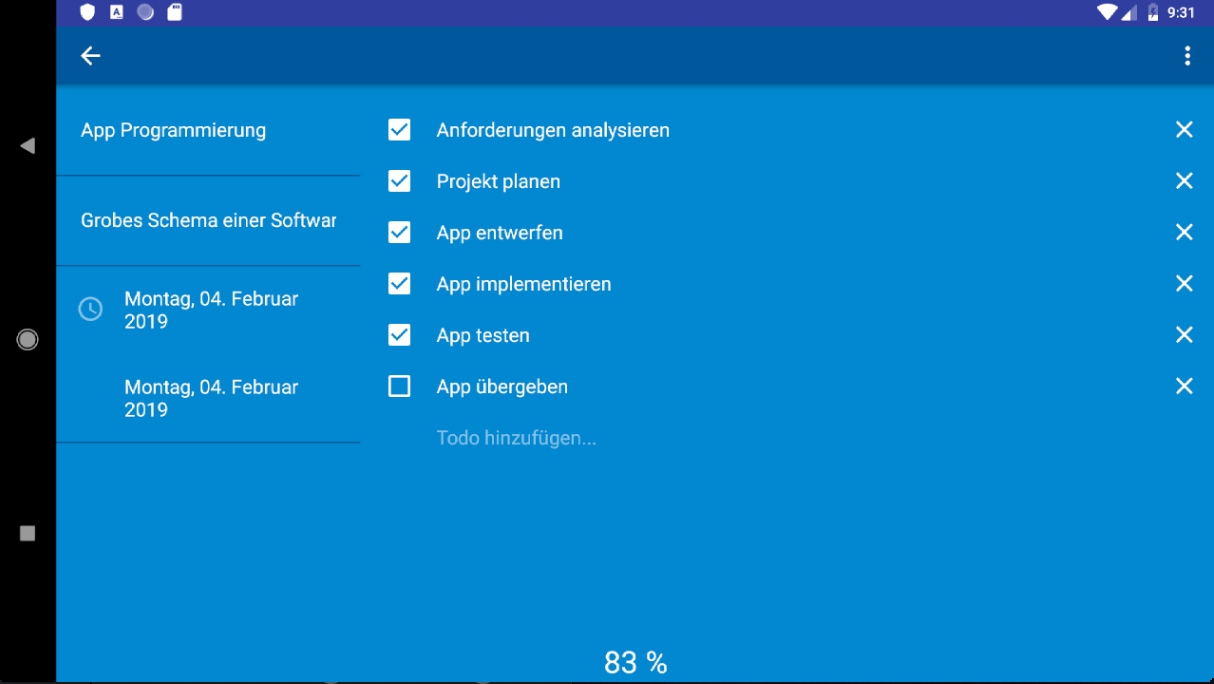
\includegraphics[width=1\textwidth]{img/Todo_landscape}\\ % Pfad
\source{Screenshot aus der Benutzeroberfläche} % Quelle
\end{minipage}
\end{figure}

Beim Wechsel der beiden Ansicht-Modi werden die Daten jeweils in das andere Layout übernommen.

\begin{figure}[H]
\centering
\begin{minipage}[t]{1\textwidth} % Breite, z.B. 1\textwidth		
\caption{Todo Activity im Portrait-Modus} % Überschrift
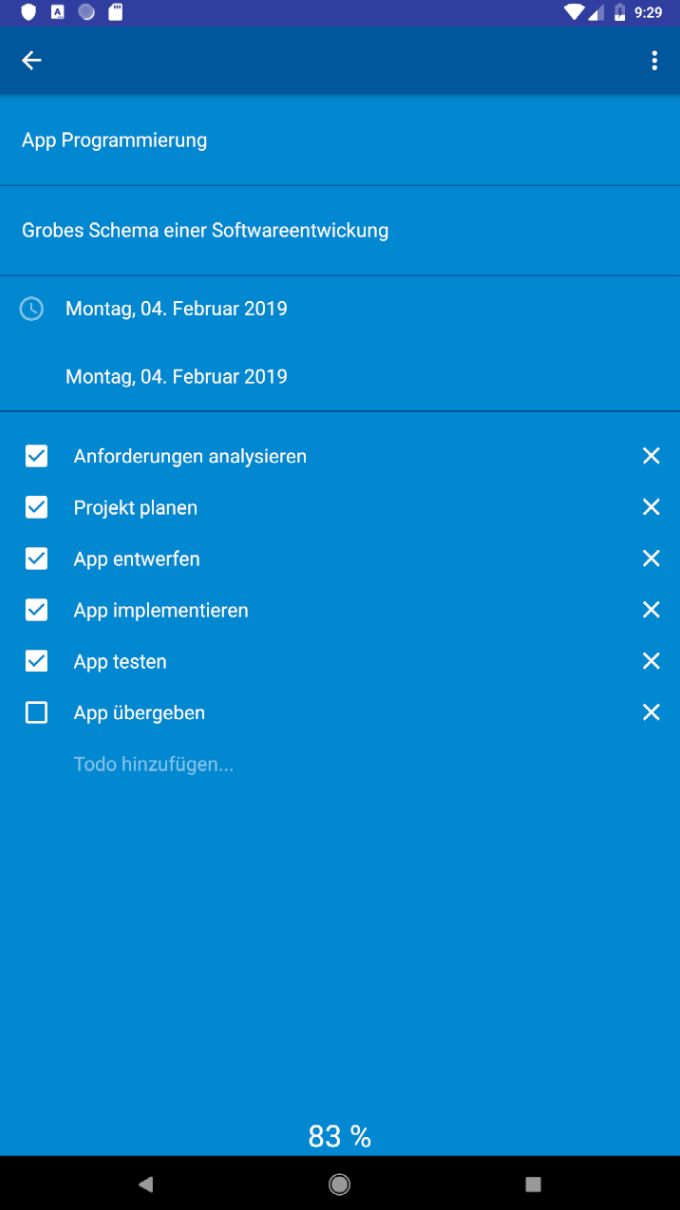
\includegraphics[height=20cm]{img/Todo_portrait}\\ % Pfad
\source{Screenshot aus der Benutzeroberfläche} % Quelle
\end{minipage}
\end{figure}

Nachdem auf eines der Eingabefelder für Daten getippt wurde, initialisiert die Activity einen Datepicker und zeigt dem Benutzer ein gewohntes Auswahlmenü für ein gewünschtes Datum an. Dies hat den Vorteil, dass der Benutzer durch Erfahrungen in anderen Apps schnell und einfach mit der Datumeingabe zurechtfindet. Wie im Screenshot zu sehen ist, kann der Benutzer mit „Abbrechen“ die Datumsauswahl abbrechen, sodass das Eingabefenster geschlossen wird. Mit dem „Ok“-Button hat der Benutzer alternativ die Möglichkeit, seine Eingabe zu übernehmen. Hierbei liest die Activity das eingegeben Datum aus und stellt es formatiert dar. Es wird außerdem indem Todo-Objekt zwischengespeichert.

\begin{figure}[H]
\centering
\begin{minipage}[t]{1\textwidth} % Breite, z.B. 1\textwidth		
\caption{Datumeingabe} % Überschrift
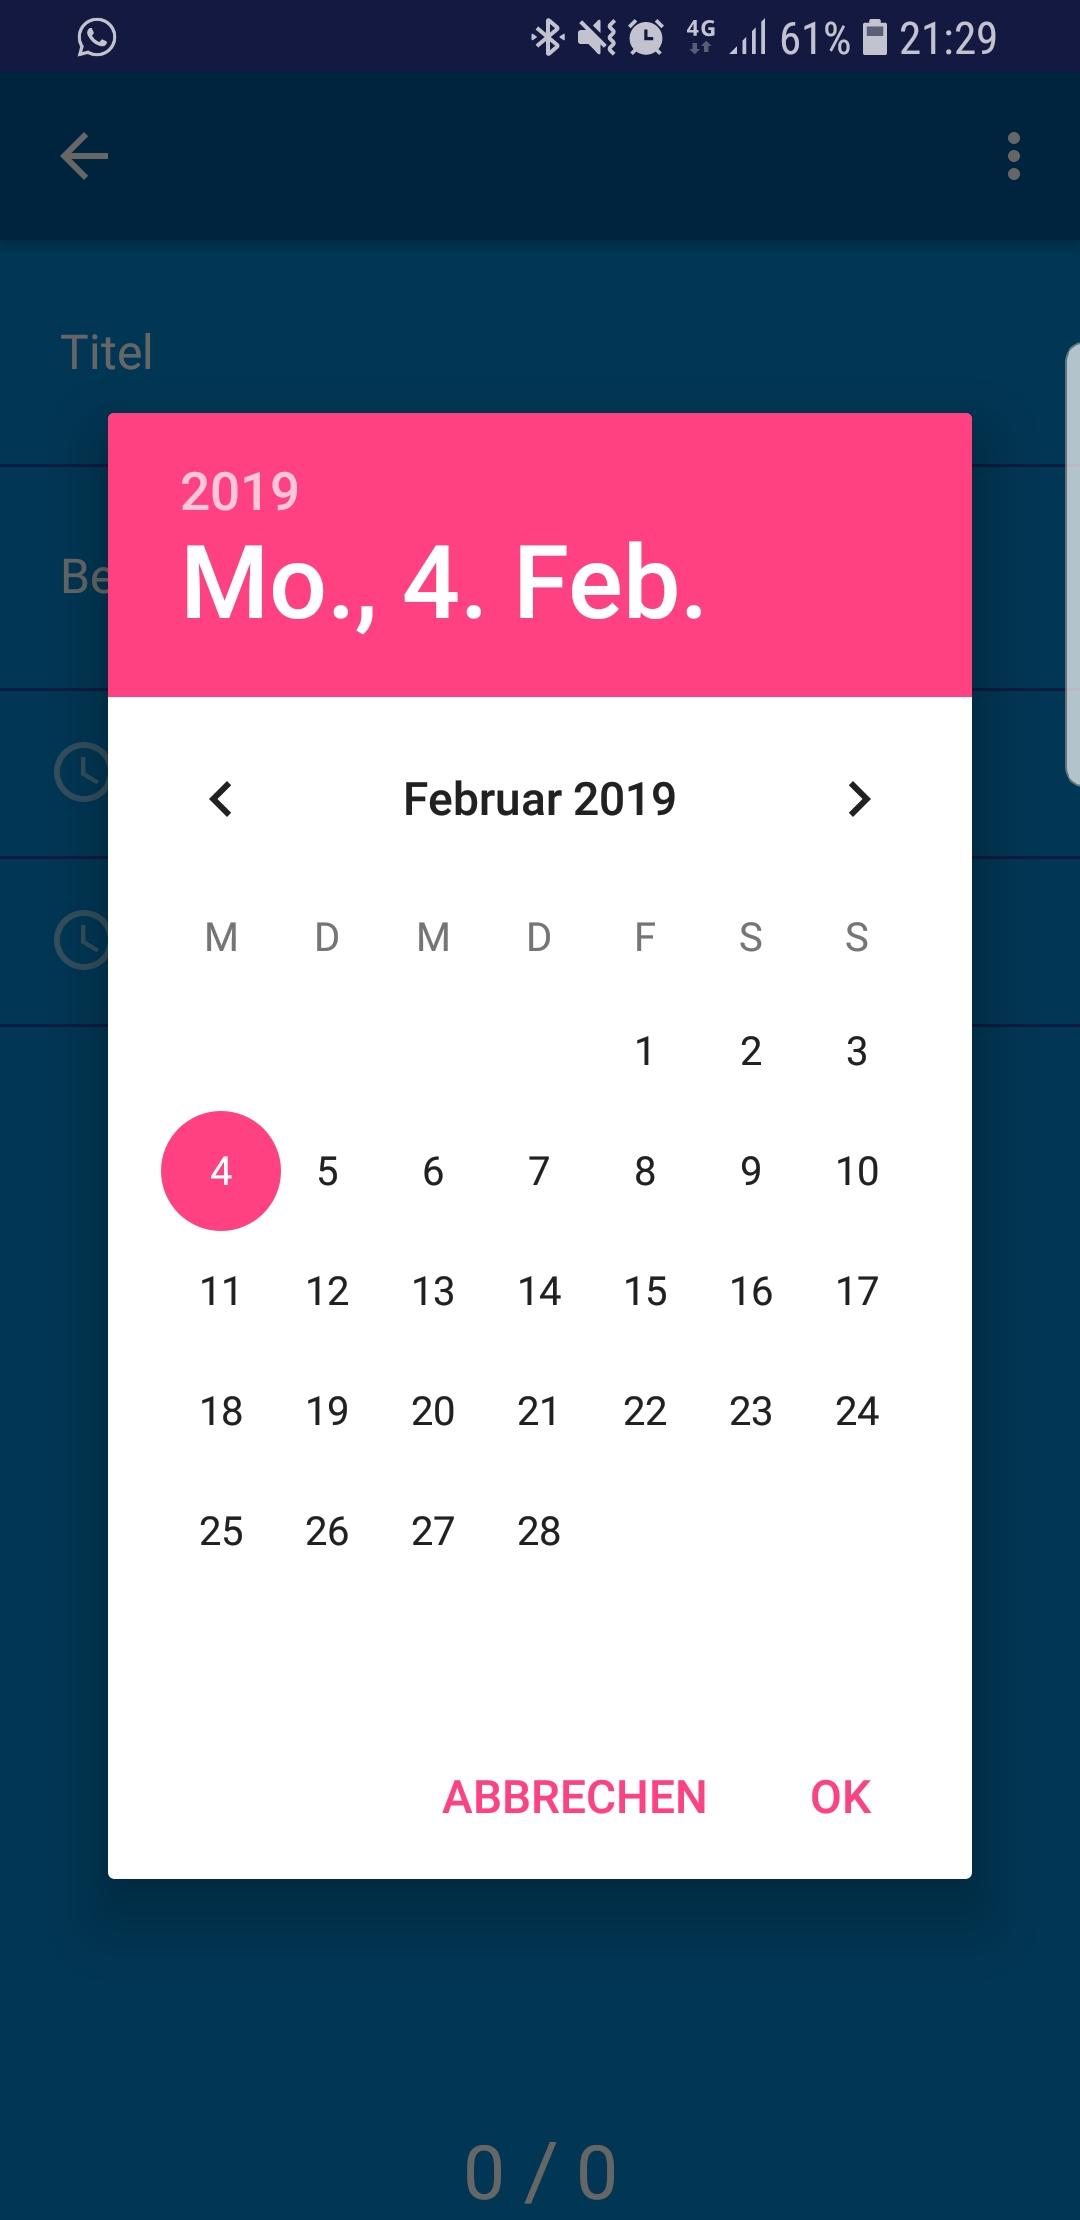
\includegraphics[height=20cm]{img/Todo_Datepicker}\\ % Pfad
\source{Screenshot aus der Benutzeroberfläche} % Quelle
\end{minipage}
\end{figure}

%Florian
\paragraph{Use Case (Florian Rath)}
Die Todo-Activity kann man über zwei Wege erreichen. Beide Wege erfolgen aus der Übersichts-Activity.

Der User kann entweder eine neue Todo erstellen, sodass in der Todo-Activity eine nicht vorhandene Todo-ID übergeben wird, oder er kann auf eine bereits vorhandene Todo tippen. Die ID dieser Todo wird dann aus der Datenbank geladen und in der Activity dargestellt. Die Todo-Activity deckt die Funktionalitäten des Todo-TEN‘s ab.

%Sertan
\paragraph{Datenstrukturen und -typen (Sertan Cetin)}
Um die gewünschten Anforderungen zu erfüllen und dabei sowohl eine hohe Wartbarkeit als auch Modularität zu gewährleisten, wurden innerhalb der Todo-Activity mehrere Klassen implementiert. Nachfolgend werden diese Klassen vorgestellt.

Wenn die Todo-Activity aus der Overview-Activity gestartet wird, wird eine Instanz der Klasse Init, die die Schnittstelle AppCompatActivity implementiert, erstellt. In dieser Klasse werden weitere Klassen, die im Rahmen des Projektes angelegt wurden, erstellt. Bei diesen Klassen handelt es sich um Gui, TodoApplicationLogic und Data. Auf diese wird im Nachfolgenden näher eingegangen.

Die Gui-Klasse ist die Schnittstelle zum Layout. Hier werden alle Layout-Elemente in Variablen bzw. typgleichen Objekten gespeichert. So wird z.B. das Eingabefeld für den Titel in einer Variablen vom Datentyp EditText gespeichert. Indem jedes Element aus dem Layout in einer Variablen hinterlegt wird, erhält man die Möglichkeit diese vom Java-Code aus auszulesen bzw. zu manipulieren. Diese Klasse besitzt einen Konstruktor, in welchem die eigentliche Erstellung der genannten Objekte geschieht. Über Getter- und Setter-Methoden stellt die Gui-Klasse den anderen Klassen die Schnittstelle zum Layout zur Verfügung.

Die Data-Klasse speichert das Todo und stellt die Schnittstelle zwischen der Datenbank und der Applikationslogik dar. Sie ist somit für das Speichern, Löschen und Ändern verantwortlich. Im Konstruktor dieser Klasse wird außerdem das Todo-Objekt initialisiert. Beim Initialisierungsvorgang der Data-Klasse wird eine ID übergeben. Ist diese ID nicht vorhanden, wird legt sie ein neues Todo in der Datenbank an. Andernfalls wird das Todo geladen.

In der TodoApplicationLogic-Klasse findet die gesamte Geschäftslogik statt. Sie verbindet im Wesentlich die Data mit der Gui. Sie ist unteranderem für die Interaktion zuständig.

\paragraph{Dokumentation des Quelltextes der Activity}
In diesem Kapitel wird der Quelltext der Todo-Activity vorgestellt und erläutert. Dabei wird Klasse für Klasse, Methode für Methode vorgegangen. 
Methoden der Init-Klasse (Sertan Soner Cetin)
Die Init Klasse verfügt insgesamt über 10 Methoden. Da die Klasse die Schnittstelle AppCompatActivity implementiert, sind die Methoden onCreate, onCreateOptionsMenu, onSaveInstanceState, onActivityResult, onBackPress und onConfigurationChanged vorhanden. Daneben sind noch Methoden wie initData, initGUI und initApplicationLogic vorhanden.
Private void initApplication() 
Diese Methode initialisiert das Objekt des Typs TodoApplicationLogic. Diese ApplicationLogic erhält die GUI- und Data-Objekte
Private void initData(String todoId)
Diese Methode initialisiert das Data-Objekt des Datentyps Data. Das Objekt erhält eine Instanz zur Activity und eine Todo-ID vom Typ String, welche dieser Methode ebenfalls übergeben wird.
Private void initGui()
Diese Methode initialisiert das Gui-Objekt. Dieses Objekt erhält eine Instanz zu der Activity.
Public void onCreate(Bundle savedInstanceState)
Diese Methode wird beim Erstellvorgang der Init-Klasse aufgerufen. Sie ruft die zuvor beschriebenen Methoden auf. Der Parameter savedInstanceState wird der Oberklasse übergeben.
Methoden der Gui-Klasse (Sertan Soner Cetin)
Die Gui-Klasse verfügt über einen Konstruktor, der im vorangegangenen Kapitel beschrieben wurde. Außerdem verfügt sie über diverse Getter- und Setter-Methoden. Es werden einige exemplarisch dargestellt.
Public void setFocusableInTouchmode(boolean value)
Diese Methode stellt den TouchModus des Layouts aus. Über den Parameter value kann angegeben werden, ob sich die Tastatur beim Start des Layouts aufklappen soll oder nicht. (true für nicht ausklappen, false für ausklappen)
Public EditText getmTitle()
	Diese Getter-Methode liefert das Objekt mTitle des Datentyps EditText zurück.
Public void setmTitle(string pTitle)
Diese Setter-Methode schreibt in das Textfeld des Todo-Layouts den übergebenen Parameter mit dem Namen pTitle des Datentyps String.
Public EditText getmText()
Diese Getter-Methode liefert das Objekt mText des Datentyps EditText zurück. Das Objekt entspricht dem Layout-Element für die Beschreibung des Todos.
Public void setColor(int color, int darkColor)
An diese Methode werden zwei Farbwerte als Integer übergeben. Der erste Farbwert entspricht einem helleren Farbton, z.B. Hellblau. Der zweite wäre ein dunklerer Blauton, z.B. Dunkelblau. Das Layout bekommt die helle Farbe als Hintergrundfarbe, während die Toolbar oder Trennlinien zwischen den einzelnen Elementen die dunklere Farbe erhalten.
Methoden der Data-Klasse (Sertan Soner Cetin)
Diese Klasse verfügt über einen Konstruktor und über Getter- und Setter-Methoden. Durch die Schnittstelle zur Datenbank sind noch Methoden für das Löschen und Ändern der Todo in der Datenbank vorhanden.
Public void deleteTodo()
	Löscht die Todo aus der Datenbank anhand seiner ID.
Public void updateTodo()
	Ändert die Todo in der Datenbank und aktualisiert somit alle Eigenschaften.
Public void setTitle(string title)
Ändert den Titel der Todo. Der Parameter title des Datentyps String ist der neue Titel.
Public boolean getmIsNew()
Gibt an, ob die Todo neuerstellt wurde oder beim Start der Activity bereits vorhanden war. Dieser Wert wird außerhalb benötigt, um festzulegen, ob sich die Tastatur beim Activity-Start aufklappen soll oder nicht.
Methoden der TodoApplicationLogic (Florian Rath)
Die TodoApplicationLogic stellt die größte Klasse innerhalb der Todo-Activity dar. Dies liegt unter anderem daran, dass die meisten Verantwortlichkeiten hier liegen. Sie ist Dreh und Angelpunkt der gesamten Infrastruktur, da sie die Data bzw. Datenbank mit der Gui bzw. dem Layout verbindet und alles steuert.
Private void initGui()
Diese Methode stellt die Gui ein und ruft eine andere Methode namens dataToGui auf.
Private void dataToGui()
Diese Methode schreibt die Todo-Eigenschaften auf die einzelnen Layout-Elemente. So wird z.B. der Todo-Titel in das Eingabefeld für den Titel geschrieben oder die Farbe des Todos als Hintergrundfarbe festgelegt.
Private void initListener()
Da innerhalb der Applikationslogik die Listener für die einzelnen Events z.B. ClickEvent oder TouchEvent verwaltet werden, wurde diese Methode angelegt, um alle Listener an einer zentralen Stelle zu initialisieren. Hier werden der ClickListener, TouchListener und CheckedChangeListener initialisiert und bei den einzelnen Layout-Elementen registriert.
Public void receiveDate(Date date)
Diese Methode wurde für den Datepicker benötigt. Sie empfängt quasi das Datum aus dem Eingabefeld. Der Parameter date wird dann an das Eingabefeld übergeben.
Public String formatDate(Date date)
Diese Methode liefert einen String zurück. Der Parameter date wird in eine leserliche Formatierung gebracht. Die Formatierung des Datums ist z.B. „Dienstag, 13. Januar 2019“.
Public void showDatePickerDialog(View v)
Diese Methode initialisiert das DatePickerFragment. Dazu wird der Parameter v benötigt, um die beiden Start- und Enddatum-Felder unterscheiden zu können, da beide denselben DatePicker verwenden.
Public void returnToOverview()
Diese Methode leitet den Benutzer wieder zur Overview-Activity zurück. Bei diesem Vorgang wird außerdem die UpdateTodo-Methode aufgerufen, die weiter unten beschrieben ist.
Public void onMenuItemClick(MenuItem item)
Bei dieser Methode handelt es sich um einen Event-Handler. Diese wird ausgeführt, wenn ein Menü-Item angeklickt wird. Da nur ein Menüpunkt vorhanden ist, ist es eindeutig. An dieser Stelle wird die externe Methode des Data-Objekts deleteTodo aufgerufen. Außerdem wird die zuvor beschriebene returnToOverview-Methode aufgerufen.
Public void createList()
Diese Methode erzeugt eine Liste bzw. initialisiert den TaskAdapter. Der TaskAdapter wird benötigt, um aus einer Liste von Tasks in eine ListView-Elementliste zu verwandeln. Dieser Adapter wird dem GUI-Element ListView zugewiesen.
Private void addTask()
Diese Methode fügt Tasks-Liste, welche in der GUI angezeigt wird, ein Element hinzu.
Public void updateProgress()
Die updateProgress-Methode holt sich aus dem Todo-Objekt den Anteil der erledigten Aufgaben. Dieser Wert wird in eine Prozentzahl umgewandelt. Der Prozentwert wird dem entsprechenden Layout-Element zugewiesen.
Private void onEditTextClicked()
Bei dieser Methode handelt es sich um einen Event-Handler. Dieser wird ausgeführt, wenn auf ein EditText-Feld getippt wurde. Dabei wird ein neues EditText-Feld erzeugt, um eine weitere Aufgabe eingeben zu können.
Public void onActivityReturned(int requestCode, int resultCode, Intent data)
	Diese Methode deckt den Fall ab, falls in die Activity zurückgekehrt wird.
Private void onDelteButtonClicked(int id)
Es wird dieser Methode eine ID übergeben. Diese ID entspricht der Aufgabe, bei der der Lösch-Button geklickt wurde. Anhand dieser ID wird der Task aus der Liste entfernt.
Private void onTextChanged(String s, View mView)
Bei dieser Methode handelt es sich um einen Text-Changed Event-Handler. Der Parameter s steht für den Text und mView für das Element. Handelt es sich um den Titel, wird die setTitle-Methode des Data-Objekts aufgerufen. Handelt es sich um die Beschreibung, wird die setText-Methode desselbigen Objekts aufgerufen.
Public void onOkButtonClicked()
Wenn der OK-Buttons des Datumeingabefelds geklickt wird, wird die Methode UpdateTodo aufgerufen.
Public void onBackPressed()
Wird der Zurück-Button aus der Toolbar gedrückt, wird die UpdateTodo-Methode aufgerufen. So wird beim Verlassen der Activity die Todo in der Datenbank gespeichert.
Private void addInputTaskField()
Fügt der Task-Liste ein weiteres Element hinzu. Außerdem wird der TaskAdapter benachrichtigt, um die GUI zu aktualisieren. Hierdurch wird auch der prozentuale Anteil der erledigten Aufgaben beeinflusst, weshalb die Methode updateProgress aufgerufen wird.
Public ArrayList<Task> getmTasks()
Liefert die ArrayList mit Task-Objekten zurück.
Private int getTasksItemCount()
Liefert eine Zahl zurück, die angibt, wie viele Elemente in der Task-Liste gespeichert sind.
Public ClickListener getClickListener()
Gibt das ClickListener-Objekt zurück.
Public TouchListener getTouchListener()
	Gibt das TouchListener-Objekt zurück.
Public CheckedChangeListener getmCheckedChangeListener()
	Gibt das CheckedChangeListener-Objekt zurück.
Public void UpdateTodo()
Diese Methode speichert zuerst das Todo-Objekt aus der Data-Klasse in einer lokalen Todo-Methodenvariable. Von diesem werden der Titel und Beschreibung gesetzt. Das Start- und Enddatum werden ebenfalls aktualisiert. Am Ende der Methode wird das Todo in der Datenbank gespeichert bzw. aktualisiert.
Public void onConfigurationChanged(Gui pGui)
Bei dieser Methode handelt es sich um einen Event-Handler. Diese initialisiert die Gui und Listener erneut. Dazu werden die beschriebenen Methoden initGui und initListener aufgerufen.

\newpage
\subsubsection{Event Activity (Robin Menzel)}
\fancyhead[L]{Event Activity}
%Robin
Dieses Kappitel beschreibt die Funktionsweise der Event-Ansicht innerhalb des TEN-Managers. Diese wird aufgerufen, wenn ein Event aus der Übersichtsseite angeklickt wird oder ein neues Event erstellt wird.

\paragraph{Aufgaben und Funktionen}

Die \textit{Event Activity} hat die Funktion eine Übersicht über ein Event zu geben, Bearbeitungen zu dem Event zu verarbeiten, oder ein neues Event zu erstellen und speichern. Möchte ein User eine neues Event erstellen, ist die Event-Activity bis auf das aktuelle Datum leer. In den Textfeldern stehen halbtransparente Hinweise, wie "Titel eingeben", die dem User Hinweise über den Inhalt geben. Wenn die Activity ein bereits vorhandenes Event anzeigt, kann durch ein Klick auf die jeweilige Konfiguration, eine Änderung durchgeführt werden.

Ganz oben ist eine Toolbar zu finden, welche zum einen eine Navigation zurück zur Übersichtsseite bietet und zum anderen ein Options/Drei-Punkt Menü beinhaltet. Durch einen Klick auf das 3-Punkt Menu der \textit{Event Activity}  kann das Event in Form von Text per E-Mail oder Chat-Applikation geteilt werden. Auch ein Export in eine andere Kalender-Applikation wird hier unterstützt. Die letzte Option bietet das Löschen des Events an.

Da ein Event immer ein Datum und eine Zeit hat, kann auch dieses in der Activity ausgewählt werden. Über einen Klick auf das Datum oder die Uhrzeit, öffnet sich ein Dialog Picker, über den sich die Uhrzeit oder das Datum auswählen lässt.

Bestimmte Events wie Geburtstage wiederholen sich in bestimmten Intervallen. Auch diese Events lassen sich in der Activity abbilden, in dem unter der Zeit auf (initialer Wert) Einmalig geklickt wird. Hier steht dem User die Option Einmalig, Täglich, Wöchentlich und Jährlich zur Verfügung. Angezeigt wird immer der Termin, der am nächsten liegt.

Sobald ein User mehr als einen Buchstaben in die Adresszeile des Events eingibt, leuchtet das Navigationsicon auf. Ein klick auf dieses öffnet sich Google Maps und versucht den eingegeben Ort zu finden.

Als letzte Option lassen sich Erinnerungen zu diesem Event einstellen. Dazu hat der User eine Wahl zwischen 1 Stunde vorher, 6 Stunden vorher, 1 Tag vorher und 1 Woche vorher. Es lassen sich kein, ein, mehrere, oder alle Erinnerungen auswählen. Liegt der Zeitpunkt der Erinnerung in der Zukunft, so wird zu diesem Zeitpunkt eine Push-Benachrichtigung auf dem Gerät erscheinen, welche den Titel und die Uhrzeit des Events enthält.

\paragraph{Layout}

Das Layout der Activity setzt sich aus verschieden Komponenten zusammen:
\begin{itemize}
\item \textit{activity\_event.xml}
\item \textit{toolbar\_ten.xml}a
\end{itemize}
Bei \textit{activity\_event.xml} handelt es sich um ein Drawer Layout. Es beinhaltet die Toolbar \textit{toolbar\_ten.xml}. Die Inhalte sind in einem Scroll View zusammengefasst.

Die Toolbar \textit{toolbar\_ten.xml} ist für alle TENs identisch und beinhaltet ein Drei-Punkt-Menu mit den Menüpunkten aus \textit{event\_menu.xml}
\begin{itemize}
\item Event teilen
\item Event in den Kalender
\item Event löschen
\end{itemize}

\begin{figure}[H]
\centering
\begin{minipage}[t]{1\textwidth} % Breite, z.B. 1\textwidth		
\caption{Screenshot - Event Activity} % Überschrift
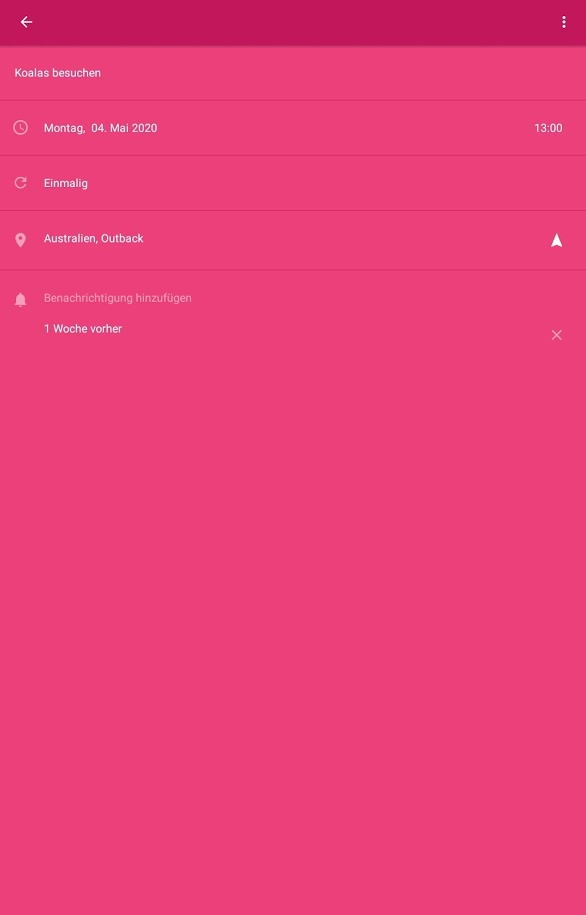
\includegraphics[width=13 cm]{img/Screenshot_EventActivity.jpg}\\ % Pfad
\source{Screenshot aus der Benutzeroberfläche} % Quelle
\end{minipage}
\end{figure}

\begin{figure}[H]
\centering
\begin{minipage}[t]{1\textwidth} % Breite, z.B. 1\textwidth		
\caption{Screenshot - Event Activity Erinnerung} % Überschrift
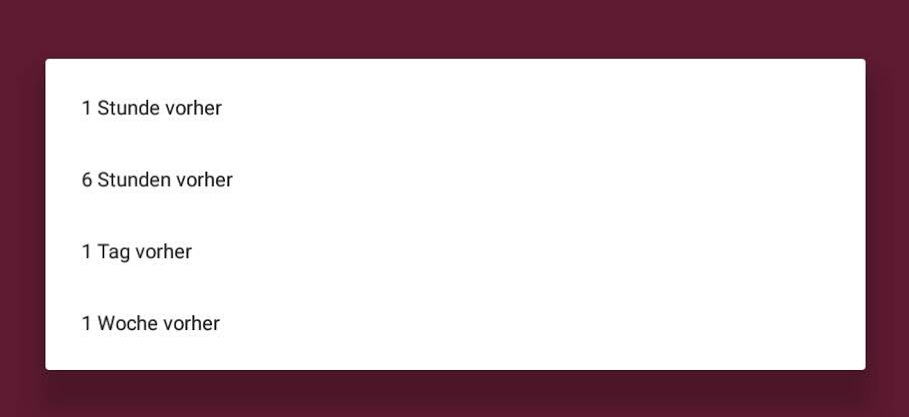
\includegraphics[width=13 cm]{img/Screenshot_EventActivityReminder.jpg}\\ % Pfad
\source{Screenshot aus der Benutzeroberfläche} % Quelle
\end{minipage}
\end{figure}

\begin{figure}[H]
\centering
\begin{minipage}[t]{1\textwidth} % Breite, z.B. 1\textwidth		
\caption{Screenshot - Event Activity Wiederholung} % Überschrift
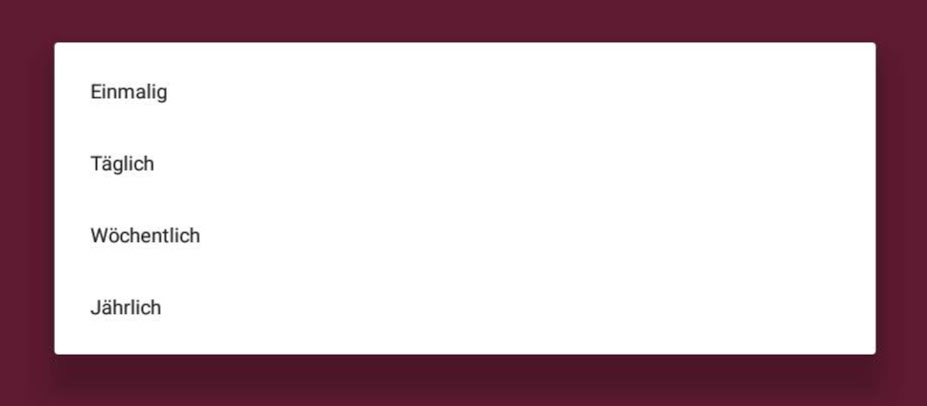
\includegraphics[width=13 cm]{img/Screenshot_EventActivityRecurringType.jpg}\\ % Pfad
\source{Screenshot aus der Benutzeroberfläche} % Quelle
\end{minipage}
\end{figure}

\begin{figure}[H]
\centering
\begin{minipage}[t]{1\textwidth} % Breite, z.B. 1\textwidth		
\caption{Screenshot - Event Activity Toolbar} % Überschrift
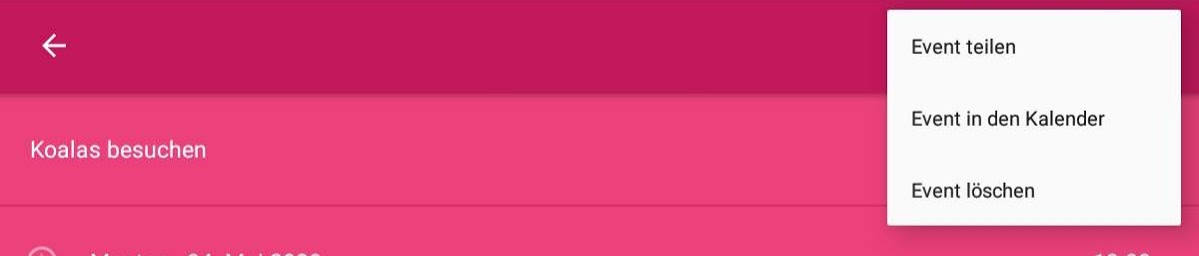
\includegraphics[width=13 cm]{img/Screenshot_EventActivityToolbar.jpg}\\ % Pfad
\source{Screenshot aus der Benutzeroberfläche} % Quelle
\end{minipage}
\end{figure}

\paragraph{Use-Case}
Diese Activity dient dem User hauptsächlich zum Anlegen, Bearbeiten, Ansehen und Löschen von einem Event. Außerdem ist die Activity verantwortlich für alle Reminder, die als Push-Benachrichtigung erscheinen und an das jeweilige Event erinnern. In der Activity ist es des Weiteren möglich, über einen Button Google Maps inklusive der Adresse des Events zu öffnen und so zu dem Event zu Navigieren. Außerdem ist es möglich das Event in Form von Text zu teilen (z.B. per E-Mail oder Textnachricht) oder in eine Kalender Applikation zu übertragen.

\begin{figure}[H]
	\centering
	\caption{Use-Case - Event Activity}
	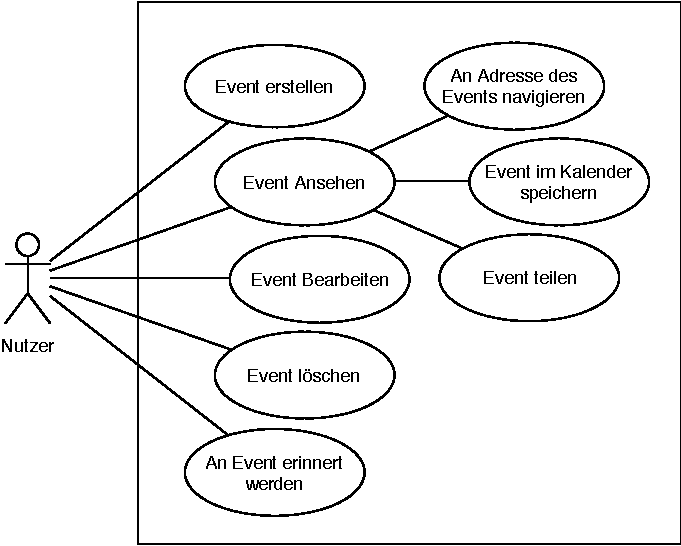
\includegraphics[width=12cm]{img/EventActivityUseCase.pdf}
	\label{img:EventActivityUseCase}
\end{figure}

\paragraph{Datenstruktur und -typen}
Die \textit{Event Activity} wird aus der \textit{MainActivity} mittels eines Intents gestartet, welcher falls das Event bereits besteht und kein neues Event angelegt werden soll, die jeweilige ID des Events übergibt, um darüber auf die Datenbank zuzugreifen. Die Klasse EventActivit ist aus der Klasse AppCompatActivity abgeleitet und überschreibt die für die Funktionen relevanten Methoden diese Klasse und initialisiert die im Nachfolgenden angesprochenen Verwaltungsklassen EventData, EventGui und EventApplicationLogic.

Die Event-Activity selbst ist in mehrere Pakete aufgeteilt um innerhalb der insgesamt 14 Klassen für eine übersichtliche Struktur zu sorgen und die einzelnen Klassen ihren übergeordneten Funktionen zuzuordnen. Die Funktionen der einzelnen Klassen und die Klasseninteraktion sind in der Dokumentation des Quelltextes am Ende dieses Kapitels dargestellt.

\subparagraph{Logic Paket}
Das Paket welches die Logik der \textit{Event Activity} beinhaltet, beinhalten alle Listener und Watcher Klassen und die \textit{EventApplicationLogic}. Damit ist sie die zentrale Logik-Klasse der Activity. Von hier aus werden die andren Klassen, welche spezifische Aufgaben übernehmen, initialisiert und angesprochen. Zu den anderen Klassen gehören die Klassen zur Erneuerung der GUI, des automatischen Speichern von Änderungen und den Klassen zur Verwaltung von Erinnerungen.

\subparagraph{Data-Paket}
Das Data-Paket beinhaltet alle Klassen welche für die Datenhaltung zuständig sind. Zentrale Klasse ist hier die \textit{EventData-Klasse} welche für das Laden, aber auch das Speichern von Änderungen bzw. neuen Events zuständig ist. Zudem beinhaltet das Data-Paket eine Reminder Klassse, welche dafür sorgt, dass Reminder zum einen als Zeitpunkt der Erinnerung, aber auch in Text-Form (``1 Stunde vorher'') genutzt werden kann. \\
Die \textit{Event Activity} interagiert neben der \textit{Overview Activity} auch mit anderen Apps. Entweder durch die ShareAction oder durch die Google Maps Intents.

\subparagraph{Gui-Paket}
Innerhalb des Gui-Paketes subd alle Klassen einsortiert, welche die für die Darstellung der GUI verantwortlich sind. Die EventGui Klasse repräsentiert die Struktur des Layouts und damit alle einzelnen Komponenten, um diese korrekt zu initialisieren und auf einzelne Views zugreifen zu können. Außerdem enthält das Paket die Dialog Picker TimePicker und DatePicker, die für die Auswahl eines Datums bzw. einer Uhrzeit zuständig sind. Zu guter letzt hilft die RecurringTypeHelper dabei die Wiederholungen als Zahlen, aber auch in Textform (``Einmalig'') abbilden zu können.

\paragraph{Dokumentation des Queltextes der Activity}
Im Nachfolgenden sind die einzelnen Klassen der \textit{Event Activity} mit den jeweiligen wichtigsten Funktionen kurz beschrieben.
\subparagraph{EventActivity}
Diese Klasse ist der zentrale Einstiegspunkt der Note-Activity und ist aus der AppCompatActivity-Klasse abgeleitet. Hier werden eineige Methoden dieser Klasse überschrieben und an die neuen Anforderungen angepasst.

\textit{onCreate}:\\
Die Activity wird durch einen Intent von der \textit{Overview Activity} gestartet, welchem die ID für ein Event mitgegeben wurde. Diese ID wird ausgelesen und anhand dieser die Event-Data Klasse initialisiert. Zusätzlich wird die EventGui und die EventApplicationLogic Klasse initialisiert.

\textit{onBackPressed}:\\
In dieser Methode wird das normale vorgehen ersetzt durch die Funktion returnToOverview der EventApplicationLogic um wieder in die Overview-Klasse zurückzukehren.

\textit{onCreateOptionsMenu}:\\
In dieser Methode wird das Menü mit dem Event Menü gefüllt.\\

\subparagraph{LOGIC}
\subparagraph*{EventApplicationLogic}
Diese Klasse ist die zentrale Logik der Activity.\\
\\
\textit{updateGui}\\
Diese Methode setzt alle Werte aus dem Event-Objekt aus der EventData Klasse in die aktuelle Gui ein.\\
\\
\textit{returnToOverview}\\
Mit Hilfe dieser Methode wird die Activity verlassen und kehrt zurück zur Overview Activty.\\
\\
\textit{setAlarm}\\
Wenn ein Reminder erstellt wird, wird hier der Zeitpunkt zum AlarmManager hinzugefügt (solange der Zeitpunkt in der Zukunft liegt).\\
\\
\textit{updateReminder}\\
Wenn sich die Zeit verändert, müssen auch die Zeitpunkte der Reminder angepasst werden. Dies geschieht in dieser Methode.\\
\\
\textit{onNewReminderClicked}\\
Diese Methode kümmert sich um das Erstellen eines neuen Reminders, solange noch nicht alle vier möglichen Reminder hinzugefügt wurden.\\
\\
\textit{onTextChanged}\\
Sobald der Textwatcher ausgelöst wird, wird diese Funktion aufgerufen um das Event Objekt dynamisch zu speichern.\\
\\
\textit{onCloseReminderClicked}\\
Diese Methode kümmert sich um das Löschen einer Reminders. Dazu gehört auch, diesen aus dem Alarm Manager zu entfernen.\\
\\
\textit{onMenuItemClicked}\\
Diese Methode wird aufgerufen, sobald auf einen der drei Menüpunkte geklicked wurde.\\
\\
\textit{onNavicationIconClicked}\\
Wurde auf das Icon neben der Adresse geklickt, so erstellt diese Funktion einen Google Maps Intent, der die Adresse in Google Maps öffnet.\\
\\
\textit{onRecurrinTypeClicked}\\
Diese Funktion öffnet einen AlertDialog in welchem man den Wiederholungstypen auswählen kann.

\subparagraph{listener Klassen}
Die listener Klassen in dem LOGIC Paket erben alle von View.onClickListener, text.TextWatcher und Toolbar.onClickListener. In ihnen wird differenziert welches Element den Listener ausgelöst hat und führt dementsprechend eine Methode aus.


\subparagraph{DATA}
\subparagraph*{EventData}
In dieser Klasse findet die komplette Datenhaltung statt.\\
\\
\textit{updateEvent}\\
In dieser Methode wird des Services ``Update'' der Datenbank genutzt um ein Event-Objekt zu speichern.\\
\\
\textit{deleteEvent}\\
In dieser Methode wird des Service ``Delete'' der Datenbank genutzt um ein Event-Objekt zu löschen.\\
\\
\textit{shareEvent}\\
Diese Methode wird Aufgerufen falls der User im ein Event teilen möchte. Von hier aus wird die shareEvent-Methode im ShareModule aufgerufen.\\
\\
\textit{getFormateDate}\\
Diese Methode gibt das Datum des Events in sprach-formattierung zurück, wie z.B. 25. Januar 2019.\\
\\
\textit{exportToCalendar}\\
Diese Methode erstellt aus dem Event ein Intent, welches von allen gängigen Kalender Applikationen untersützt und geöffnet werden kann.\\
\subparagraph{Reminder}
Diese Klasse hilft beim Umgang mit Remindern. So müssen z.B. Reminder neu berechnet werden, wenn sich die Zeit des Events verändert hat.\\
\\
\textit{getLabelFromReminder}\\
Diese Methode gerrechnet aus der Differenz zwischen dem Zeitpunkt der Erinnerung und dem Zeitpunkt des Events die Beschriftung (z.B. ``1 Stunde vorher'').\\
\\
\textit{getReminderFromLabel}\\
Diese Methode errechnet aus der Beschrifftung den richtigen Zeitpunkt einer Erinnerung.

\subparagraph{GUI}
\subparagraph*{EventGui}
Diese klassse beinhaltet alle Benutzeroberflächenattribute, auf welche so zugegriffen werden kann.\\
\\
\textit{setColor}\\
Die bunte Farbgestalltung ist ein Kernelement unseres Designs. Daher enthält jedes TEN-Objekt auch feste Farbattribute, welche beim Aufbau der Gui dargestellt werden müssen. Diese Methode weißt aus den Farbwerten des Event-Objektes, den Gui Elementen ihre spezifische Farbe zu.\\
\\
\textit{setReminder}\\
Diese Klasse stellt die Reminder, die im Event-Objekt nur als Zeitpunkte dargestellt sind, auf der Oberfläche da. Dafür interagiert diese mit der Reminder Klasse und passt auch das Auswahl-Menü für weitere Reminder an.

\subparagraph{DatePicker und TimePicker}
Diese Klassen sind fast identisch. Sie erben von der Klasse DialogFragment und überschreiben notwendige Methoden.\\
\\
\textit{onCreateDialog}\\
In dieser Methode wird ein Calendar Objekt erstellt um in ihm später die Ausgewählten Zeiten zu speichern. Falls bereits eine Zeit existiert, wird diese übernommen. Anschließend wird ein DatePickerDialog erstellt.\\
\\
\textit{onDateSet} oder \textit{onTimeSet}\\
Falls eine Zeit ausgewählt wurde, ruft diese Methode, die entsprechenden Methoden in der EventApplicationLogic auf und übergibt die ausgewählten Zeite.\\
\\
\textit{setTime}\\
Da über einen Konstruktor eine vorhandene Zeit eines Events noch nicht übergeben werden kann, muss der Date/Time-Picker zuerst erstellt werden und anschließend kann über diese Methode die bereits vorhandene Zeit eingestellt werden.

\subparagraph{RecurringTypeHelper}
Diese Funktion stellt eine Verbindung zwischen dem Enum Objekt ReccuringType und den Beschriftungen der Wiederholungen her.

\newpage
\subsubsection{Note Activity}
\fancyhead[L]{Note Activity}
FHDW

\newpage
\fancyhead[L]{}
\subsection{Dokumentation der Navigation zwischen Activities (Yannick Rüttgers)}
%%%%%%%%%%%
%Yannick
%%%%%%%%%%%

Der Einstiegspunkt für den Nutzer ist die OverviewActivity. Von dieser aus können alle weiteren Activities aufgerufen werden, wie in der Planungsphase geplant.

Die Activities werden auf zwei Arten aufgerufen. Entweder geschieht dies, um ein neues TEN zu erstellen, oder um ein bereits vorhandenes aufzurufen.

Soll ein neues TEN erstellt werden, geschieht dies über einen der drei Buttons am oberen Bildschirmrand. Je nachdem welche TEN-Art angeklickt wurde, wird eine dazugehörige Activity erstellt und ohne Mitgabe weiterer Parameter aufgerufen.

Wenn hingegen ein bereits bestehendes TEN angezeigt werden soll, wird wieder die dazugehörige Activity erstellt. Diesmal wird der Activity allerdings als Parameter die ID des TENs weitergeben. Das Laden dessen übernimmt dann die jeweilige Activity.

Wenn aus den einzelnen TEN-Activities zurücknavigiert wird, gelangt der Nutzer zurück in die Übersichtsactivity. Die TENs innerhalb dieser werden neu geladen, um eventuelle Veränderungen anzeigen zu können.

\subsection{Dokumentation der Activity-übergreifenden, persistenten Datenhaltung (Jan Beilfuß)}
%%%%%%%%%%%
%Jan
%%%%%%%%%%%

\subsubsection{Objekte}
Im Bereich der persistenten Datenspeicherung gab es die Herausforderung, dass es eine brei-te Auswahl an Speichermöglichkeiten gibt. Es musste zu Beginn evaluiert werden, welche Technologie für das Projekt am geeignetsten war. Zur Auswahl standen Bundles und Daten-banken, welche sich weiter in SQL-Datenbanken und NoSQL-Datenbanken unterteilen las-sen. Darüber hinaus war zu Projektbeginn nicht bekannt, welche Datenbankimplementierun-gen für den Einsatz auf mobilen Geräten geeignet sind. Nach einiger Recherche wurde die Implementierung im Bundle als zu aufwendig und nicht flexibel genug erachtet. In der Folge wurde sich für den Einsatz einer Datenbank entschieden.

Aus dem bisherigen Studienverlauf waren unter den Datenbanken nur SQL-Datenbanken bekannt. Diese unterscheiden sich von NoSQL-Datenbanken, indem man eine klare Daten-struktur, in der Regel in Tabellenform vorgibt. NoSQL-Datenbanken sind beispielsweise do-kumenten- oder graphenbasiert. Dokumente sind flexibel und diesen können einfache Felder in Form von Key-Value-Paaren hinzugefügt werden. Im mobilen Umfeld hat man häufig Än-derungen am Datenmodell, sodass einem in diesem Bereich eine NoSQL-Datenbank entge-gen kommt. Weiterhin hat man bei SQL-Datenbanken einen Aufwand zur Erzeugung und Definition von Tabellen sowie bei deren Änderung. Und da man aus den Anforderungen an die App ableiten konnte, dass keine komplexen Tabellenrechnungen gefordert waren, wurde sich für eine dokumentenbasierte NoSQL-Datenbank entschieden. 

Bei der Wahl der spezifischen Datenbanktechnologie entschied man sich am Ende für Couchbase Lite, da diese gut dokumentiert ist, einem eine lokale Datenbank und Tools wie ein Gateway zur Hand gibt, wenn man es langfristig in Erwägung zieht Todos, Events und Notizen über einen Server zu synchronisieren.

Um den Aufwand bei der Umwandlung von Java-Objekten zu Dokumenten zu vereinfachen, wurde das Serialisierungs- und Deserialisierungsframework Jackson verwendet. Dieses wan-delt Java Objekte in JSON-Strings um, welche in jeweils einem Dokument abgelegt wurden. Weiterhin bietet es eine Funktionalität, diese wieder zurückzuwandeln. Einige Attribute, darun-ter die ID des TEN-Objektes, die Hauptfarbe, die Kontrastfarbe und das Erzeugungsdatum wurden hiervon ausgenommen. Die ID ist die ID des Dokumentes selber und würde somit doppelt gehalten werden. Die Farben wurden in eigenen Key-Value-Paaren abgelegt, damit man nicht das gesamte TEN-Objekt erzeugen muss, wenn man auf diese zugreifen möch-te.Dies fand Einsatz in der Note Activity. Hier war es das Ziel die Performance beim Öffnen zu optimieren. Daher wurden die Farben getrennt von den eigentlichen Notizdaten im Vorraus geladen. Weiterhin wurde im Dokument gespeichert, welche Klasse das zuspeichernde Ob-jekt hat, damit dieses beim Laden vernünftig aus dem JSON-String erzeugt werden kann. Zusätzlich wurden noch die Objektattribute welche bei Datenbankabfragen genutzt wurden, in einem eigenen Key-Value-Pair abgespeichert.

\subsubsection{Bilder}
Das Speichern der Bilder hat sich im Vergleich zu den Java-Objekten als aufwendiger erwie-sen, da diese mehr Speicherplatz und Rechenleistung benötigen.

Der erste Lösungsansatz war, die Bilder als Binary Large Objects in der Datenbank abzule-gen. Dies erwies sich als zu imperformant und umständlich, sodass entschieden wurde, die Bilder im Dateisystem des Gerätes zu speichern. Weiterhin wurde zwischen den Bildern in hoher Auflösung und Bildern in Vorschaugröße unterschieden. Die Vorschaubilder werden in der Übersicht und Notiz-Activity eingebunden. Aufgrund der stärkeren Kompression und ge-ringeren Auflösung können diese schneller geladen werden. Darüber hinaus ist es auf dem Zielgerät hardwarebedingt nicht möglich, mehrere Bilder in Originalgröße im Arbeitsspeicher zu halten.

\newpage
\subsection{Dokumentation der Activity-übergreifenden Klassen (Ruthild Gilles)}
%%%%%%%%%%%
%Ruthild
%%%%%%%%%%%

Zu den Activity-übergreifenden Klassen gehören abgesehen von den Query-Klassen für die persistente Datenhaltung auch die Service-Klassen und die Models-Klassen. Die Models-Klassen enthalten die TEN-Klasse und die einzelnen Todo-, Event- und Note-Klassen. Hier sind auch weitere Util-Klassen untergeordnet. In den Service-Klassen sind Methoden enthalten, die die Schnittstelle zwischen Datenbank und Activities darstellen. Im Folgendem wird genauer auf die einzelnen Klassen eingegangen.

\subsubsection{Models-Klassen}

\subsubsection{Service-Klassen}

Damit die Activities die Daten der TEN-Objekte auf der dokumentenbasierten Datenbank speichern können, wurden Service Klassen implementiert. Hierzu gehörten hauptsächlich Klassen zum Erzeugen neuer TEN-Objekte (Create), zum Erhalten bereits gespeicherter TEN-Objekte von der Datenbank (Read), zum Speichern veränderter TEN-Objekte (Update) und zum Löschen von TEN-Objekten von der Datenbank (Delete). Diese sogenannte CRUD-Operationen wurden in den entsprechenden Klassen teilweise für alle drei verschiedenen Objekttypen einzeln eingefügt, teilweise aber auch für TEN-Objekte im Allgemeinen. Dank Polymorphie können die jeweils einzelnen Objekttypen ebenfalls an die entsprechenden Methoden übergeben werden.

Diese Struktur wurde während der Planungsphase vom Datenteam überlegt und während der Implementierung angepasst. Wie auch schon in der Planungsphase definiert enthält die Create-Klasse Methoden, die ein neues leeres Todo, Event oder Note zurückgeben. Diese Methode ruft den Konstruktor der jeweiligen TEN-Klasse auf. Eine Interaktion mit der Datenbank ist hier noch nicht nötig.

Die Read-Klasse hingegen muss auf die Datenbank zugreifen, um entweder alle TEN-Objekte an die Main-Activity in einem ListArray zu übergeben oder aber ein spezielles Todo, Event oder Note, welches von den einzelnen Todo-, Event- oder Note-Activities aufgerufen werden kann. Damit das gewünschte TEN-Objekt in der Datenbank gefunden werden kann, benötigen die Read-Methoden die ID des gewünschten Objektes. Dieses wird als String beim Aufruf der jeweiligen Methode übergeben.

Die Update-Klasse dient zum Speichern von Änderungen an Todo-, Event- und Note-Objekten. Dazu überprüft die Methode, der ein TEN-Objekt übergeben wurde, ob dieses bereits auf der Datenbank existiert. Ist dies der Fall, wird eine Methode zum Ausführen des Update-Befehls auf der Datenbank aufgerufen. Ist dies nicht der Fall, wird eine Methode zum Ausführen des Insert-Befehls auf der Datenbank aufgerufen. Da die Todo-, Event- und Note-Klassen von der TEN-Klasse erben, kann hier Polymorphie angewandt werden. Es ist nur eine Methode zum Speichern notwendig.

Für das Löschen von TEN-Objekten sind in der Delete-Klasse zwei Methode vorhanden. Die eine löscht nur ein übergebenes TEN-Objekt aus der Datenbank, indem es eine entsprechende Methode aus einer der Repository-Klassen aufruft und dieser die ID des TEN-Objektes übergibt. Sollen jedoch mehrere TEN-Objekte auf einmal gelöscht werden, kann der zweiten Methode eine Array List, die mehrere zu löschende Objekte enthält, übergeben werden. Dabei müssen die Objekte nicht alle von dem gleichen Datentyp sein, sondern können Todo-, Event- und Note-Objekte enthalten. Die Methode iteriert durch die übergebene Array List und ruft für jeden Eintrag die Methode zum Löschen eines Objektes auf.


